\documentclass[12pt,twoside]{report}
\usepackage{lmodern}
\usepackage{amssymb,amsmath}
\usepackage{ifxetex,ifluatex}
\usepackage{fixltx2e} % provides \textsubscript
\ifnum 0\ifxetex 1\fi\ifluatex 1\fi=0 % if pdftex
  \usepackage[T1]{fontenc}
  \usepackage[utf8]{inputenc}
\else % if luatex or xelatex
  \ifxetex
    \usepackage{mathspec}
    \usepackage{xltxtra,xunicode}
  \else
    \usepackage{fontspec}
  \fi
  \defaultfontfeatures{Mapping=tex-text,Scale=MatchLowercase}
  \newcommand{\euro}{€}
\fi
% use upquote if available, for straight quotes in verbatim environments
\IfFileExists{upquote.sty}{\usepackage{upquote}}{}
% use microtype if available
\IfFileExists{microtype.sty}{%
\usepackage{microtype}
\UseMicrotypeSet[protrusion]{basicmath} % disable protrusion for tt fonts
}{}
\usepackage[margin=1in]{geometry}
\usepackage{graphicx}
\makeatletter
\def\maxwidth{\ifdim\Gin@nat@width>\linewidth\linewidth\else\Gin@nat@width\fi}
\def\maxheight{\ifdim\Gin@nat@height>\textheight\textheight\else\Gin@nat@height\fi}
\makeatother
% Scale images if necessary, so that they will not overflow the page
% margins by default, and it is still possible to overwrite the defaults
% using explicit options in \includegraphics[width, height, ...]{}
\setkeys{Gin}{width=\maxwidth,height=\maxheight,keepaspectratio}
\ifxetex
  \usepackage[setpagesize=false, % page size defined by xetex
              unicode=false, % unicode breaks when used with xetex
              xetex]{hyperref}
\else
  \usepackage[unicode=true]{hyperref}
\fi
\hypersetup{breaklinks=true,
            bookmarks=true,
            pdfauthor={},
            pdftitle={},
            colorlinks=true,
            citecolor=blue,
            urlcolor=blue,
            linkcolor=magenta,
            pdfborder={0 0 0}}
\urlstyle{same}  % don't use monospace font for urls
\setlength{\parindent}{0pt}
\setlength{\parskip}{6pt plus 2pt minus 1pt}
\setlength{\emergencystretch}{3em}  % prevent overfull lines
\setcounter{secnumdepth}{0}

%%% Use protect on footnotes to avoid problems with footnotes in titles
\let\rmarkdownfootnote\footnote%
\def\footnote{\protect\rmarkdownfootnote}

%%% Change title format to be more compact
\usepackage{titling}

% Create subtitle command for use in maketitle
\newcommand{\subtitle}[1]{
  \posttitle{
    \begin{center}\large#1\end{center}
    }
}

\setlength{\droptitle}{-2em}
  \title{}
  \pretitle{\vspace{\droptitle}}
  \posttitle{}
  \author{}
  \preauthor{}\postauthor{}
  \date{}
  \predate{}\postdate{}

\usepackage[english,brazilian]{babel} % suporte para línguas
\usepackage[utf8]{inputenc} % codificação

\usepackage{subfig, epsfig}
\captionsetup[subfigure]{style=default, 
  margin=0pt, parskip=0pt, hangindent=0pt, indention=0pt, 
  singlelinecheck=true, labelformat=parens, labelsep=space}

\usepackage{ae}
\usepackage{aecompl}
\usepackage{booktabs}
\usepackage[T1] {fontenc}

\usepackage{footnote}

% Notas criadas nas tabelas ficam no fim das tabelas
\makesavenoteenv{tabular}

\usepackage{fancyhdr}

\fancypagestyle{plain}
{
  \fancyhf{}%
  \renewcommand{\headrulewidth}{0pt}%
  \fancyfoot[LE,RO]{\thepage}
}

\usepackage{graphicx,wrapfig} % para incluir figuras
\usepackage[all]{xy} % para incluir diagramas
\usepackage{amsfonts, amssymb, amsthm, amsmath, amscd, textcomp} % pacote AMS
\usepackage{color, float, bbm, multicol, rotating}
\usepackage{verbatim, listings, booktabs}

\usepackage{caption} % Customizar as legendas de figuras e tabelas
\usepackage{array} % Elementos extras para formatação de tabelas

\usepackage[switch,pagewise]{lineno} % números nas linhas

\usepackage {tocvsec2} % controlar profundidade de table of contents
\setcounter {secnumdepth}{0}
\setcounter {tocdepth}{1}

%\widowpenalty10000
%\clubpenalty10000

% \usepackage{mathpazo} % fonte palatino
\usepackage{baskervald} % fonte com cara de manuscrito 1920
\usepackage{hyperref}

% Adicionar bibliografia, índice e conteúdo na Tabela de conteúdo
% Não inclui lista de tabelas e figuras no índice
\usepackage[nottoc,notlof,notlot, notindex]{tocbibind}

\usepackage{icomma} % Posicionar inteligentemente a vírgula como separador decimal
\usepackage[tight]{units} % Formatar as unidades com as distâncias corretas

\usepackage{setspace}

\usepackage{lastpage} % Conta o número de páginas

\usepackage{pdflscape} % ambiente landscape

\usepackage[round]{natbib}
\usepackage{chapterbib}

\usepackage[flushleft]{threeparttable}
\usepackage {tabularx}

\usepackage{pdfpages}

\usepackage{fixme}
%\usepackage{pdfcomment}

\fxsetup{layout={footnote}}

% --- definições gerais ---
\newcommand{\barra}{\backslash}
\newcommand{\To}{\longrightarrow}
\newcommand{\abs}[1]{\left\vert#1\right\vert}
\newcommand{\set}[1]{\left\{#1\right\}}
\newcommand{\seq}[1]{\left<#1\right>}
\newcommand{\norma}[1]{\left\Vert#1\right\Vert}
\newcommand{\hr}{\par\noindent\hrulefill\par}
% --- ---

\newcommand{\titulo}{Perspectivas sobre o reconhecimento de padrões de modularidade e suas implicações para a evolução de morfologias complexas}
\newcommand{\nomedoaluno}{Guilherme Garcia}
\newcommand{\advisor}{Gabriel Marroig} \newcommand{\ano}{2015}
\hypersetup{colorlinks=true, linkcolor=black, citecolor=black,
  filecolor=black, pagecolor=black, urlcolor=black,
  pdfauthor={\nomedoaluno}, pdftitle={\titulo}, pdfsubject={Genética e
    Biologia Evolutiva}, pdfkeywords={Genética Quantitiva, Morfologia
    Craniana, Roedores}, pdfproducer={Latex}, pdfcreator={pdflatex}}
 
\geometry{bindingoffset=20pt}

%\geometry{paperwidth=290mm, paperheight=297mm, margin=1in}
%\setlength{\marginparwidth=80mm}

\setcounter{topnumber}{1}
\setcounter{bottomnumber}{1}
\setcounter{totalnumber}{1}
\renewcommand{\topfraction}{0.7}
\renewcommand{\bottomfraction}{0.3}
\renewcommand{\textfraction}{0.335}
\renewcommand{\floatpagefraction}{0.5}

\setlength{\headheight}{15pt}


\begin{document}

\maketitle


\pagestyle{empty}

\clearpage
\hbox{}
\newpage
% Capa
\begin{center}
\par
\Huge {\nomedoaluno} \\
\vspace\fill
\Huge {\bf \titulo} \\
\vspace\fill \Large {On the recognition of modularity patterns and its implications for the morphological evolution of complex phenotypes} \\
\vspace\fill
\includegraphics[width=10cm]{Figures/spiral} \\
\vspace\fill
{\bf{\large São Paulo}\\
  {\large \ano}}
\end{center}

\clearpage
\hbox{}
\newpage

\pagestyle{plain}

% Números das páginas em algarismos romanos
\pagenumbering{roman}

% Página de Rosto
\begin{center}
\Huge{\nomedoaluno}
\par
\vspace\fill
\Huge {\bf \titulo}
\end{center}
\par
\vspace\fill \hspace*{150pt}\parbox{10cm}{{\large Tese
    apresentada ao Instituto de Biociências da Universidade de São
    Paulo, para a obtenção de Título de Doutor em Ciências, na Área de
    Genética e Biologia Evolutiva.}}

\par
\vspace {1 cm}
\hspace*{150pt}\parbox{10cm}{{\large Orientador: \advisor}}

\par
\vspace\fill
\begin{center}
\textbf{{\large São Paulo}\\
{\large \ano}}
\end{center}

\newpage

% Ficha Catalográfica
\begin {center}
Ficha Catalográfica \\
\fbox{
  \begin{minipage}{10cm}
    Garcia, Guilherme

    \hspace{2em} \titulo.

    \hspace{2em} \pageref{LastPage} páginas.
    
    \hspace{2em}Tese (Doutorado) - 
    Instituto de Biociências da Universidade de São Paulo. 
    Departamento de Genética e Biologia Evolutiva.
    
    \begin{enumerate}
    \item Evolução Morfológica;
    \item Morfologia Craniana;
    \item Modularidade;
    \item Integração Morfológica;
    \item Primatas Antropóides.
    \end{enumerate}
    I. Universidade de São Paulo. 
    Instituto de Biociências. 
    Departamento de Genética e Biologia Evolutiva.
  \end{minipage}
}
\par
\vspace\fill
{\LARGE\textbf{Comissão Julgadora:}}

\par
\vspace\fill
\begin{tabular*}{\textwidth}{@{\extracolsep{\fill}}l l}
\rule{16em}{1px} 	& \rule{16em}{1px} \\
Prof. Dr. 		& Prof. Dr. \\
 & \\
\end{tabular*}

\par
\vspace\fill
\begin{tabular*}{\textwidth}{@{\extracolsep{\fill}}l l}
\rule{16em}{1px} 	& \rule{16em}{1px} \\
Prof. Dr. 		& Prof. Dr. \\
 & \\
\end{tabular*}

\par
\vspace\fill

\parbox{16em}{\rule{16em}{1px} \\
Prof. Dr. \advisor}
\end{center}

\newpage

% Dedicatória
% Posição do texto na página
\vspace*{0.75\textheight}
\begin{flushright}
  \emph{Para Moisés e Ramiro.}
\end{flushright}

\newpage

% Epígrafe
\vspace*{0.2\textheight}
{\noindent 
If only I could \\
Clear my eyes \\
Then I might breathe once more \\
Then I might breathe again \\
\vspace{0.2 cm} \\
Old sun and stars, \\
And oceans below me \\
Guide my strides over \\
Jagged shards, under foot \\
\vspace{0.2 cm} \\
To slash to the sound \\
How many sit on woe or peril? \\
How many walk on their own? \\
\vspace{0.2 cm} \\
Into the truth \\
Let myself burn \\
Now it's written \\
1000 shards \\
\vspace{0.2 cm} \\
\emph {Isis - 1000 Shards}
}

\newpage
\begin{flushright}
\footnotesize{\noindent 
Black \\
then \\
white are \\
all I see \\
in my infancy. \\
Red and yellow then came to be \\
reaching out to me. \\
Lets me see. \\
\vspace{0.2 cm}
There is \\
so \\
much more \\
and beckons me \\
to look through to these \\
infinite possibilities. \\
As below \\
so above and beyond \\
I imagine. \\
Drawn outside the lines of reason. \\
Push the envelope. \\
Watch it bend. \\
\vspace{0.2 cm}
Over thinking, over analyzing \\
separates the body from the mind. \\
Withering my intuition \\
leaving opportunities behind. \\
\vspace{0.2 cm}
Feed my will to feel this moment \\
urging me to cross the line. \\
Reaching out to embrace the random. \\
Reaching out to embrace whatever may come. \\
\vspace{0.2 cm}
I embrace my desire to \\
feel the rhythm, to feel connected \\
enough to step aside and weep like a widow \\
to feel inspired, to fathom the power, \\
to witness the beauty, to bathe in the fountain, \\
to swing on the spiral, to swing on the spiral, \\
to swing on the spiral of our divinity \\
and still be a human. \\
\vspace{0.2 cm}
With my feet upon the ground \\
I lose myself between the sounds \\
and open wide to suck it in. \\
I feel it move across my skin. \\
I'm reaching up and reaching out. \\
I'm reaching for the random \\
or whatever will bewilder me. \\
Whatever will bewilder me. \\
And following our will and wind \\
we may just go where no one's been. \\
We'll ride the spiral to the end \\
and may just go where no one's been. \\
\vspace{0.2 cm}
Spiral out. Keep going. \\
\vspace{0.2 cm}
\emph{Tool - Lateralus}
}
\end{flushright}

\newpage

% Agradecimentos

% Espaçamento duplo

% \noindent{\LARGE\textbf{Agradecimentos}}

% \vspace{1.0 cm} 
% \emph{``If I have seen further, it is by standing in
%   the shoulder of giants.''}
% \begin{flushright}
% \emph {Isaac Newton}
% \end{flushright}
% \vspace{1.0 cm}
% \noindent{
%   \onehalfspacing

Em primeiro lugar, agradeço ao meu orientador, Gabriel Marroig, por ter me dado a oportunidade de trabalhar neste tema e por sempre contribuir para me devolver ao chão com as nossas discussões e o rigor com que ele encara a ciência. 
Espero que nós tenhamos muitos e muitos anos de colaboração pela frente.

Agradeço também aos meus pares, os demais alunos do LEM, por prover um ambiente fantástico para se fazer ciência, onde as discussões sempre acontecem, inclusive agora, aqui ao lado, enquanto escrevo estes agradecimentos. 
E claro, muitas vezes nossas discussões vão para além da ciência, mas nunca em direção ao senso comum, e estas outras conversas também contribuem ao seu modo para a confecção de um doutor em ciências.

À Aninha, por ser diversas vezes interrompida por um fluxo caótico de ideias inacabadas e ter a paciência de escutá-las, desvantagem de sentar ao meu lado.
À Paulinha, por nunca ter recusado ir tomar um café comigo, mesmo que ela precisasse muito ir embora e por toda a empolgação que ela traz em relação a tudo que a gente faz.
À Dani, pelo suprimento infinito de polenguinho light, por ler vários pedaços desta tese ainda em formação, e por todos os sorrisos e abraços que ajudaram nas horas mais escuras.
À Tafinha (ou Bárbara), por manter o bom humor mesmo nestas horas escuras e por sempre estar disposta a discutir essencialmente qualquer coisa, independente de quanto tempo isso vai levar.
À Monique, pelas divagações aleatórias a respeito de ciência, que contribuem muito pra esta tese, sem dúvida, e também pelas conversas a respeito das nossas crianças lindas.
Ao Ogro (ou Diogo), pela parceria agora de longa data nas partes mais cabeludas das análises e por ser uma fonte inesgotável de boa música, boa comida, e bom gosto em geral.
Ao Lugar (ou Fábio), pelo humor \emph{nonsense} afiadíssimo que sempre alegra o dia e pelas nossas discussões edificantes a respeito do mundo mágico da morfometria geométrica.
Ao Wally (ou Thiago), pela companhia nas tarefas mais divertidas, por exemplo levar computadores pro conserto, e claro, pelas infinitas discussões sobre ciência, sociedade e muito, muito mais.
E à Papete (ou Anna), por ser uma boa companhia pra todas as horas, da mesinha até a volta pra casa, por escutar o que eu tenho a dizer, independente do que seja, e pelas parcerias que a gente ainda deve levar em frente a respeito desses primatas aí.
Também agradeço aqueles que já deixaram o LEM, em especial Alex, Fino, Edgar e Harley, por todas as contribuições pessoais e profissionais nos anos que passaram.
Nesse embalo, agradeço também o Aríete (ou Gustavo) pelas nossas discussões regadas à café ou cerveja, que com certeza contribuem muito, e também por ler pedaços desta tese em formação.

Agradeço também aos colegas do grupo-irmão do Diogo Meyer, que ofereçem diversas perspectivas diferentes às nossas; em especial à Bárbara e ao Limão (ou Luiz Carlos), pelas conversas muito boas que tivemos recentemente. Também agradeço ao Rui Murrieta, pela oportunidade de ser monitor na disciplina de Filosofia, o que certamente contribuiu para o desenvolvimento desta tese, e ao Sérgio Matioli, por conta dos comentários durante a minha qualificação que foram o ponto de partida para o Capítulo 4. 

Agradeço à FAPESP pela concessão de uma bolsa de doutorado.

Devo também agradecer a minha família. 
Sem todos vocês, seria impossível chegar até aqui. 
Em especial, aos meus pais, Eduardo e Teresa, pelo apoio incondicional durante todos esses anos.
Ao meu irmão Gustavo, que nunca tem receios em me dizer o que eu tenho que ouvir.
E à vó Carlota, pela dieta de banana, cabeça de peixe e taboada na infância.

Finalmente, agradeço a minha companheira, a Giuliana, por estar aqui ao meu lado, mesmo nos piores momentos, e por me oferecer aquele abraço perfeito.
E ao Ramiro, nosso menininho, por conta daquele sorriso lindo que ele deu ontem quando eu cheguei em casa, e por dar tanto sentido a tudo.

\singlespacing
% }

\newpage

\vspace*{10pt}
\begin{center}
  \emph{\begin{large}Resumo\end{large}}\label{resumo}
\vspace{2pt}
\end{center}

\noindent
\par
\vspace{1em}
\noindent\textbf{Palavras-chave:} evolução morfológica, morfologia craniana, 
modularidade, integração morfológica, primatas antropóides

\newpage
\vspace*{10pt}
\begin{center}
  \emph{\begin{large}Abstract\end{large}}\label{abstract}
\vspace{2pt}
\end{center}

\selectlanguage{english}
\noindent

\par
\vspace{1em}
\noindent\textbf{Keywords:} morphological evolution, cranial morphology, 
modularity, morphological integration, anthropoid primates

\selectlanguage{brazilian}

\newpage

% Índice
\tableofcontents
%\listoffigures
%\listoftables
\newpage

\pagenumbering{arabic}

\def\sectionautorefname{Seção}
\def\chapterautorefname{Capítulo}
\def\figureautorefname{Figura}
\def\tableautorefname{Tabela}

\onehalfspacing

\pagestyle{fancy}

\renewcommand{\chaptermark}[1]{\markboth{#1}{}}
\renewcommand{\sectionmark}[1]{\markright{#1}{}}

\fancyhf{} \fancyhead[RO]{\itshape \leftmark}
\fancyhead[LE]{\itshape \rightmark} \fancyfoot[RO,LE]{\thepage}
\renewcommand{\headrulewidth}{0.5pt} \renewcommand{\footrulewidth}{0pt}

\linenumbers
\modulolinenumbers[5]

\newpage
\chapter{Introdução}
\label{ch:intro}

\begin {sidewaystable} [htp]
  \caption {Vinte e dois marcos anatômicos registrados no crânio de antropóides. As regiões e sub-regiões cranianas às quais cada marco anatômico pertence também estão indicadas. A vista na qual cada marco foi registrado está indicada por A (anterior), P (posterior) ou AP (ambas). As descrições em itálico correspondem a marcos anatômicos tomados sobre a linha sagital. \label {tab:lms}}
  \centering
  \begin {tabularx} {\textwidth} { l c p{3 cm} p{5.5 cm} X }
    \toprule
    {\bf Marco} & {\bf Posição} & {\bf Região} & {\bf Sub-região} & {\bf Descrição} \\
    \midrule
    IS & A & Face & Oral/Nasal
    & {\it interincisivo superior}
    \\
    PM & A & Face & Oral
    & sutura maxilar-premaxilar 
    \\
    NSL & A & Face & Nasal/Oral
    & {\it extremidade rostral do osso nasal} 
    \\
    NA & A & Face & Nasal/Órbita
    & {\it extremidade caudal do osso nasal (junção com o osso frontal)} 
    \\
    BR & AP & Neurocrânio & Abóbada
    & {\it sutura entre o frontal e o parietal (posição medial)} 
    \\
    PT & AP & Neurocrânio & Abóbada 
    & sutura entre o frontal e o parietal 
    \\
    FM & A & Face & Zigomático/Órbita
    & fronto-malar 
    \\
    ZS & A & Face & Oral/Zigomático/Órbita
    & sutura superior entre o zigomático e o maxilar 
    \\
    ZI & A & Face & Zigomático 
    & sutura inferior entre o zigomático e o maxilar 
    \\
    MT & A & Face & Oral
    & tuberosidade maxilar caudal ao terceiro molar 
    \\
    PNS & A & Face & Oral
    & {\it espinha caudal do nasal} 
    \\
    APET & A & Neurocrânio & Base
    & petrous temporal 
    \\
    BA & AP & Neurocrânio & Base
    & {\it ponto ventral do forame magno} 
    \\
    OPI & AP & Neurocrânio & Base/Abóbada
    & {\it ponto dorsal do forame magno} 
    \\
    EAM & A & Neurocrânio & Zigomático/Abóbada
    & meato auditivo externo rostral 
    \\
    PEAM & A & Neurocrânio & Abóbada 
    & meato auditivo esterno caudal 
    \\
    ZYGO & A & Face & Zigomático 
    & sutura entre o zigomático e o temporal 
    \\
    TSP & A & Neurocrânio & Zigómatico/Base/Abóbada
    & sutura entre o temporal o esfenoidal e o frontal 
    \\
    TS & AP & Neurocrânio & Base 
    & sutura entre o temporal e o esfenoidal 
    \\
    JP & AP & Neurocrânio & Base 
    & processo jugular 
    \\
    LD & P & Neurocrânio & Abóbada
    & {\it sutura entre o occipital e o interparietal na linha média} 
    \\
    AS & P & Neurocrânio & Abóbada 
    & sutura entre o parietal e o occipital 
    \\
    \bottomrule
  \end {tabularx}
\end {sidewaystable}

\begin{figure}[htbp]
\centering
\includegraphics{Figures/landmarks.png}
\caption{Configuração de Marcos Anatômicos. As linhas conectando os
marcos indicam os caracteres considerados, tanto sob a forma de
distâncias euclidianas quanto variáveis locais de forma. Linhas
pontilhadas e tracejadas indicam a associação dos caracteres às
hipóteses \emph{a priori} de integração (Face e Neurocrânio,
respectivamente). \label{fig:landmarks}}
\end{figure}

\begin {table}[hp]
  \centering
  \caption {As 38 distâncias euclidianas calculadas sobre os marcos anatômicos e as regiões e sub-regiões às quais cada caráter pertence. \label{tab:dist}}
  
  \hr
  \begin {tabularx} {\textwidth} {X X X}
    \bf{Distância} & \bf{Região} & \bf{Sub-região}  \\
    \hline
    IS.PM & Face & Oral \\
    IS.NSL & Face & Nasal \\
    IS.PNS & Face & Oral/Nasal \\
    PM.ZS & Face & Oral \\
    PM.ZI & Face & Oral \\
    PM.MT & Face & Oral \\
    NSL.NA & Face & Nasal \\
    NSL.ZS & Face & Nasal \\
    NSL.ZI & Face & Oral/Nasal \\
    NA.BR & Neurocrânio & Abóbada \\
    NA.FM & Neurocrânio & Órbita \\
    NA.PNS & Face & Nasal \\
    BR.PT & Neurocrânio & Abóbada \\
    BR.APET & Neurocrânio & Abóbada \\
    PT.FM & Neurocrânio & Órbita \\
    PT.APET & Neurocrânio & Abóbada \\
    PT.BA & Neurocrânio & Abóbada \\
    PT.EAM & Neurocrânio & Abóbada \\
    PT.ZYGO & Face & Zigomático \\
    FM.ZS & Neurocrânio & Órbita \\
    ZS.ZI & Face & Oral \\
    ZI.MT & Face & Oral \\
    ZI.ZYGO & Face & Zigomático \\
    ZI.TSP & Face & Zigomático \\
    MT.PNS & Face & Oral \\
    PNS.APET & Neurocrânio & Base \\
    APET.BA & Neurocrânio & Base \\
    APET.TS & Neurocrânio & Base \\
    BA.EAM & Neurocrânio & Base \\
    EAM.ZYGO & Face & Zigomático \\
    ZYGO.TSP & Face & Zigomático \\
    LD.AS & Neurocrânio & Abóbada \\
    BR.LD & Neurocrânio & Abóbada \\
    OPI.LD & Neurocrânio & Abóbada \\
    PT.AS & Neurocrânio & Abóbada \\
    JP.AS & Neurocrânio & Base \\
    BA.OPI & Neurocrânio & Base \\
  \end {tabularx}
  \hr
\end {table} % sk:tab:dist

\begin{figure}[htbp]
\centering
\includegraphics{Figures/phylo_model-1.pdf}
\caption{Tamanhos amostrais e efeitos fixos controlados para as 109 OTUs
de primatas antropóides. \label{fig:phylo_model}}
\end{figure}

\def\sectionautorefname{Section} \def\chapterautorefname{Chapter}
\def\figureautorefname{Figure} \def\tableautorefname{Table}

\selectlanguage{english}

\newpage
\chapter{Modularity and Morphometrics: Error Rates in Hypothesis Testing}
\label{ch:modcomp}

\section{Abstract}\label{abstract}

The study of modularity in morphological systems has increased in the
past twenty years, parallel to the popularization of geometric
morphometrics, which has led to the emergence of different criteria for
detecting modularity on landmark data. However, compared to usual
covariance matrix estimators, Procrustes estimators have properties that
hinder their use. Here, we compare different representations of form,
focusing on detecting modularity patterns defined \emph{a priori}; we
also compare two metrics: one derived from traditional morphometrics
(MHI) and another that emerged in the context of landmark data (RV).
Using Anthropoid skulls, we compare these metrics over three
representations of form: interlandmark distances, Procrustes residuals,
and local shape variables. Over Procrustes residuals, both tests fail to
detect modularity patterns, while in remaining representations they show
the distinction between early and late development in skull ontogeny. To
estimate type I and II error rates, we built covariance matrices of
known structure; these tests indicate that, considering both effect and
sample sizes, tests using MHI are more robust than those using RV.
However, both metrics have low statistical power when used on Procrustes
residuals; thus, we conclude that the influence of development and
function is poorly represented on Procrustes estimators for covariance
matrices.

\section{Introduction}\label{introduction}

Modularity is a characteristic property that biological systems exhibit
regarding the distribution of interactions between their composing
elements; that is, in a given system, subsets of elements, denominated
modules, interact more among themselves than with other such subsets
(Newman, 2006; Mitteroecker \& Bookstein, 2007; Wagner \emph{et al.},
2007). This property has been well documented at different levels of
biological organization, from the dynamics of metabolic networks (e.g.
Ravasz \emph{et al.}, 2002; Andrade \emph{et al.}, 2011) to the
structure of interactions among individuals in populations (e.g. Fortuna
\emph{et al.}, 2008) and among species in ecological communities (e.g.
Genini \emph{et al.}, 2010).

Regarding morphological systems, the concept of modularity is associated
with the framework of morphological integration (Olson \& Miller, 1958;
Cheverud, 1996a), which refers to the organization of covariances or
correlations between morphological elements and the hypotheses
concerning their relationships. In this context, modularity is related
to the uneven distribution of genetic effects over phenotypic variation
articulated through development (genotype/phenotype map; Wagner, 1996);
in a classical quantitative genetics view, these genetic effects are the
result of pleiotropy and linkage disequilibrium (Falconer \& Mackay,
1996; Lynch \& Walsh, 1998). A genotype/phenotype map composed of
clusters of genes that affect clusters of traits (with little overlap)
exhibits a modular organization; this structure is thought to emerge as
the result of selection for distinct demands (Wagner \& Altenberg, 1996;
Espinosa-Soto \& Wagner, 2010; Rueffler \emph{et al.}, 2012; Melo \&
Marroig, 2015). For instance, the decoupling between fore- and hindlimb
function in certain mammalian lineages such as bats (Young \&
Hallgrímsson, 2005) and apes (Young \emph{et al.}, 2010) is associated
with the modularization of both structures, as shown by reduced
phenotypic correlations between fore- and hindlimbs and increased
correlations between elements within these limbs.

The recognition of variational modules (Wagner \& Altenberg, 1996;
Wagner \emph{et al.}, 2007) using covariance or correlation patterns in
adult populations involves an uderstanding of the underlying
developmental and functional dynamics among morphological traits (Polly,
2008; Zelditch \& Swiderski, 2011). Skull development in mammals occurs
through a series of steps, such as neurocranial growth induced by brain
development, and growth mediated by muscle-bone interactions, with
spatiotemporal overlapping between such steps (Hallgrímsson \&
Lieberman, 2008; Herring, 2011; Cardini \& Polly, 2013). Both timing and
scope of each step is regulated by different profiles of genetic
expression exhibited by cells originated from different embryonic
precursors and their response to signaling factors expressed at the
regional level; the response to these signaling factors further changes
cell expression profiles, thus generating a feedback loop of
diferentiation (Turing, 1952; Marcucio \emph{et al.}, 2005; Meinhardt,
2008; Hallgrímsson \emph{et al.}, 2009; Franz-Odendaal, 2011; Minelli,
2011). Each step in this temporal hierarchy may be regarded as modular,
since they affect a coherent subset of tissues more so than others
(Hallgrímsson \& Lieberman, 2008), although each step affect adjoining
regions through interactions among developing tissues (Cheverud \emph{et
al.}, 1992; Lieberman, 2011; Esteve-Altava \& Rasskin-Gutman, 2014);
thus, the overlapping of such processes throughout development may
complicate their association with correlation patterns (Hallgrímsson
\emph{et al.}, 2009).

Furthermore, variation in growth rates, which emerges into size
variation (Pélabon \emph{et al.}, 2013; Porto \emph{et al.}, 2013), has
a particular importance in the context of mammalian morphological
systems. Here size variation refers to variation in both scale
(isometric variation) and scale relationships (allometric variation).
This source of variation affects the overall level of correlations
between morphological traits (Wagner, 1984; Young \& Hallgrímsson,
2005), and the magnitude of integration has important consequences for
both the evolution of mean phenotypes (Schluter, 1996; Marroig \&
Cheverud, 2005, 2010; Cardini \& Polly, 2013) and the evolution of
morphological integration itself (Oliveira \emph{et al.}, 2009; Porto
\emph{et al.}, 2009, 2013; Shirai \& Marroig, 2010).

In this context, adaptive landscapes may be the central component
governing both the stability and divergence in integration patterns, as
both stabilizing and directional selection have been shown to produce
changes in integration patterns (Jones, 2007; Arnold \emph{et al.},
2008; Jones \emph{et al.}, 2012; Melo \& Marroig, 2015). The empirical
evidence available demonstrates that both stability (e.g. Marroig \&
Cheverud, 2001; Oliveira \emph{et al.}, 2009; Porto \emph{et al.}, 2009;
Willmore \emph{et al.}, 2009) and divergence (e.g. Monteiro \& Nogueira,
2010; Grabowski \emph{et al.}, 2011; Sanger \emph{et al.}, 2012; Haber,
2015) of integration patterns are possible outcomes of the evolutionary
process. Therefore, the question of whether any of these two scenarios
is the rule or exception at macroevolutionary scales remains open,
although some theoretical and methodological differences between these
works with respect to the representation of morphological features need
to be considered.

\subsubsection{Morphometrics}\label{morphometrics}

Traditionally, morphological features have been measured using distances
among elements defined in general terms, such as ``cranial length'' or
``cranial width''. Pearson \& Davin (1924) introduced the notion that
measurements should be restricted to single osteological elements,
preferably as distances between homologous features that could be
identified in a wide taxonomic coverage. Cheverud (1982a) accomodates
this notion into the framework of morphological integration, thus
considering individual measurements over single bones as local
representations of regional phenomena, that is, the functional,
developmental and genetic interactions that produce covariances among
these elements. The influence of such interactions over covariance or
correlation matrices can be accessed by defining a subset of
measurements which are associated with particular processes and
estimating a metric that summarizes such partitioning; the null
hypothesis that this partition is undistinguishable from
randomly-defined partitions can then be tested using Monte Carlo methods
(Mantel, 1967; Cheverud \emph{et al.}, 1989).

In the past three decades, geometric morphometrics (Bookstein, 1982,
1991; Kendall, 1984; Rohlf \& Slice, 1990; Goodall, 1991) has been
consolidated as a quantitative framework for the representation of
biological shape as geometric configurations of homologous features
(landmarks; Bookstein, 1991). Two principles are central here: first,
the conceptual and statistical separation of size and shape as
components of biological form; second, the use of superimposition-based
methods (GPA: Generalized Procrustes Analysis; Rohlf \& Slice, 1990;
Goodall, 1991) for the estimation of shape statistical parameters, such
as mean shape and shape covariance structure. Procrustes estimators were
proposed as a solution to the problem that landmark configurations are
arbitrarily rotated and translated; such nuisance parameters are
impossible to estimate without any assumptions (Goodall, 1991; Lele \&
McCulloch, 2002), a situation known as the identifiability problem
(Neyman \& Scott, 1948).

Although the use of Procrustes estimators is currently widespread in
geometric morphometrics toolboxes (e.g. Klingenberg, 2011; Adams \&
Otárola-Castillo, 2013), critics have been made regarding the estimation
of both mean shape configurations (e.g. Lele, 1993; Kent \& Mardia,
1997; Huckemann, 2012) and shape covariance matrices (Walker, 2000;
Adams \emph{et al.}, 2004; Linde \& Houle, 2009; Márquez \emph{et al.},
2012). For configurations in two-dimensional space, Procrustes
estimators for mean shape perform well under isotropic landmark
covariance structure (Kent \& Mardia, 1997), a situation of null
covariances among landmarks and coordinates; however, when this
assumption does not hold, Procrustes estimates for mean shape may lose
either precision and accuracy, especially when shape variation is high
(Huckemann, 2011). The example provided by Linde \& Houle (2009)
demonstrates that when such assumption is broken shape covariance
patterns are also poorly estimated; if the unknown landmark covariance
matrix is structured due to regional differences in
covariance-generating processes, such variation might be displaced and
effectively spread out through the entire landmark configuration.

A number of alternatives for estimating shape covariance matrices have
already been suggested; some of these alternatives (e.g. Monteiro
\emph{et al.}, 2005; Theobald \& Wuttke, 2006; Linde \& Houle, 2009;
Zelditch \emph{et al.}, 2009) propose modifications to the Procrustes
analysis in order to deal with heterogeneity in landmark covariance
structure. Márquez et al. (2012) propose another definition of shape
descriptors using interpolation-based techniques (Cheverud \&
Richtsmeier, 1986; Bookstein, 1989) as a starting point. These
descriptors refer to infinitesimal expansions or retractions in
reference to a unknown mean shape (Woods, 2003) estimated at definite
locations amidst sampled landmarks. The authors argue that such
descriptors are proper local measurements of shape variation, as they
can be directly linked to biological processes that generate covariation
among morphological elements.

Despite these caveats, the use of Procrustes estimators for
investigating aspects of morphological integration has increased in the
past ten years (e.g. Klingenberg \emph{et al.}, 2004; Drake \&
Klingenberg, 2010; Goswami \& Polly, 2010; Martínez-Abadías \emph{et
al.}, 2011; Sanger \emph{et al.}, 2012). The results found by these
authors are sometimes in stark constrast with similar works using
interlandmark distances (e.g. Cheverud \emph{et al.}, 1997; Oliveira
\emph{et al.}, 2009; Porto \emph{et al.}, 2009). For instance,
Martínez-Abadías et al. (2011) found a pattern of strong integration
among partitions in human skull covariance patterns, while Oliveira et
al. (2009) and Porto et al. (2009) demonstrated that humans are among
the most modular examples of mammalian skull covariance patterns.
Likewise, while Cheverud et al. (1997) had shown that 70\% of the
pleiotropic effects are confined to either anterior or posterior
mandibular components, Klingenberg et al. (2004) has found no evidence
for a modular distribution of pleiotropic effects among the partitions
of the mouse mandible using the same strain of intercrossed mice at the
same generation. Furthermore, aside from the issues regarding Procrustes
estimators, these works also propose different methods to quantify the
effects of interactions over covariance patterns. For example,
Martínez-Abadías et al. (2011) and Sanger et al. (2012) use the RV
coefficient, a multivariate correlation coefficient defined by Escoufier
(1973) which has been used to quantify modular relationships over
landmark covariance patterns since Klingenberg (2009) has proposed its
use in this context.

\subsubsection{Objectives}\label{objectives}

In the present work, we compare the methods described by Cheverud et al.
(1989) and Klingenberg (2009) to test \emph{a priori} defined modularity
patterns using anthropoid primates as a model organism. In order to
compare the performance of these methods with respect to different
representations of form, individuals in our sample are represented both
as interlandmark distances and shape variables. Furthermore, we used an
approach based on the construction of theoretical covariance matrices;
such matrices are used in order to estimate Type I and Type II error
rates for both methods. This work aims to analyze both methods, which
have been proposed in different contexts, under the same conceptual and
statistical framework, in order to produce meaningful comparisons.

\section{Methods}\label{methods}

\subsection{Sample}\label{sample}

The database we used here (\autoref{tab:modcomp_otu}) consists of 21
species, distributed across all major Anthropoid clades above the genus
level. We selected these operational taxonomic units (OTU) from a
broader database (Marroig \& Cheverud, 2001; Oliveira \emph{et al.},
2009) in order to reduce the effects of low sample sizes over estimates
of modularity patterns. Individuals in our sample are represented by 36
registered landmarks, measured using a Polhemus 3Draw (for Platyrrhini)
and a Microscribe 3DS (for Catarrhini). Twenty-two unique landmarks
represent each individual (\autoref{fig:landmarks}, \autoref{tab:lms}),
since 14 of the 36 registered landmarks are bilaterally symmetrical. For
more details on landmark registration, see Marroig \& Cheverud (2001)
and Oliveira et al. (2009).

\begin{table}[t]
  \centering
  \begin{threeparttable}
    \caption{Twenty-one species used in the present work, along with sample sizes and linear models adjusted. \label{tab:modcomp_otu}}
    \begin{tabular}{lccr}
        \toprule
        Species & Group$^a$ & $n$ & Model$^b$ \\ 
      \midrule
        \emph{Alouatta belzebul} & P & 109 & X \\ 
        \emph{Ateles geoffroyi} & P & 78 & - \\ 
        \emph{Cacajao calvus} & P & 48 & S + X \\ 
        \emph{Callicebus moloch} & P & 93 & X \\ 
        \emph{Callithrix kuhlii} & P & 129 & - \\ 
        \emph{Cebus apella} & P & 110 & X \\ 
        \emph{Cercopithecus ascanius} & C & 61 & X \\ 
        \emph{Chiropotes chiropotes} & P & 56 & X \\ 
        \emph{Chlorocebus pygerythrus} & C & 110 & X \\ 
        \emph{Colobus guereza} & C & 140 & X \\ 
        \emph{Gorilla gorilla} & C & 115 & X \\ 
        \emph{Homo sapiens} & C & 160 & S * X \\ 
        \emph{Hylobates lar} & C & 66 & X \\ 
        \emph{Macaca fascicularis} & C & 69 & X \\ 
        \emph{Pan troglodytes} & C & 61 & X \\ 
        \emph{Papio anubis} & C & 46 & X \\ 
        \emph{Piliocolobus foai} & C & 83 & X \\ 
        \emph{Pithecia pithecia} & P & 69 & S + X \\ 
        \emph{Procolobus verus} & C & 88 & X \\ 
        \emph{Saguinus midas} & P & 50 & S \\ 
        \emph{Saimiri sciureus} & P & 87 & X \\ 
      \bottomrule
    \end{tabular}
      \begin{tablenotes}
        \footnotesize
        {
        \item[$a$] C: Catarrhini; P: Platyrrhini
        \item[$b$] S: subspecies/population; X: sex.
        }
      \end{tablenotes}
    \end{threeparttable}
  \end{table}


For each OTU, we estimated phenotypic covariance and correlation
matrices for three different types of variables: tangent space
residuals, estimated from a Procrustes superimposition for the entire
sample, using the set of landmarks described on both \autoref{tab:lms}
and \autoref{fig:landmarks} (henceforth Procrustes residuals);
interlandmark distances, described in \autoref{tab:dist}; and local
shape variables (Márquez \emph{et al.}, 2012), which are measurements of
infinitesimal log volume transformations between each sample unit and a
reference (mean) shape, based upon an interpolation function that
describes shape variation between sampled landmarks. In this context, we
used thin plate splines as interpolating functions (Bookstein, 1989). We
obtained 38 transformations corresponding to the locations of the
midpoints between pairs of landmarks used to define interlandmark
distances, in order to produce a dataset that represents shape (i.e.,
form without isometric variation; Bookstein, 1991; Zelditch \emph{et
al.}, 2004) while retaining the overall properties of the interlandmark
distance dataset, such as dimensionality for example. Furthermore, we
were able to use the same hypotheses of trait associations for both
types of variables since the position of local shape variables through
the skull mirrors the position of interlandmark distances, although they
are conceptually different types of measurements.

Here we considered only covariance or correlation structure for the
symmetrical component of variation; therefore, prior to any analysis, we
controlled the effects of variation in assymmetry. For interlandmark
distances, we averaged bilateral measurements within each individual.
For both Procrustes residuals and local shape variables, we followed the
procedure outlined in Klingenberg et al. (2002) for bilateral structures
by obtaning for each individual a symmetrical landmark configuration,
averaging each actual shape with its reflection along the sagittal
plane; we estimate local shape variables afterwards. With respect to
Procrustes residuals, landmarks placed along the sagittal plane will
have zero variation in the direction normal to this plane; we aligned
all specimens' sagittal plane to the $xz$ plane, thus removing the $y$
component for each of these landmarks from covariance/correlation
matrices.

For each dataset, we estimated covariance and correlation matrices after
removing effects of little interest in the present context, such as
sexual dimorphism, for example. For interlandmark distances and local
shape variables these effects were removed through a multivariate linear
model adjusted for each species, according to \autoref{tab:modcomp_otu};
for Procrustes residuals, the same effects were removed by centering all
group means to each species' mean shape since the loss of degrees of
freedom imposed by the GPA prohibits the use of a full multivariate
linear model over this kind of data to remove fixed effects.

In order to consider the effects of size variation on modularity
patterns we used different procedures to remove the influence of size
from each type of variable. For interlandmark distances we used the
approach established by Bookstein et al. (1985); if $\mathbf{C}$ is a
correlation matrix, we obtained a correlation matrix $\mathbf{R}$
without the effect of size using the equation

\begin{equation}
\mathbf{R} = \mathbf{C} - \lambda_1 v_1 v^{t}_1
\label{eq:iso}
\end{equation}

where $\lambda_1$ and $v_1$ refer respectively to the first eigenvalue
and eigenvector of the spectral decomposition of $\mathbf{C}$, since
this eigenvector commonly represents size variation in mammals,
especially when interlandmark distances are considered (Wagner, 1984;
Mitteroecker \emph{et al.}, 2004; Mitteroecker \& Bookstein, 2007); $t$
denotes matrix transpose.

For Procrustes residuals and local shape variables the effects of
isometric variation were removed by normalizing each individual to unit
centroid size. However, allometric relationships still influence
covariance or correlation structure. In order to remove this effect we
used a procedure based upon Mitteroecker et al. (2004), which relies on
the estimation of an allometric component $a$ for each OTU, composed of
normalized regression coefficents for each of the $m$ shape variables
(either Procrustes residuals or local shape variables) over log Centroid
Size. If $\mathbf{S}$ is a covariance matrix, we obtained a covariance
matrix $\mathbf{R}$ without the influence of allometric relationships
using the equation

\begin{equation}
\mathbf{R} = (I_m - aa^t) \mathbf{S} (I_m - aa^t)
\label{eq:allo}
\end{equation}

where $I_m$ represents the identity matrix of size $m$. Therefore, our
empirical dataset consists of six sets of covariance/correlation
matrices, corresponding to each type of morphometric variables
considering the presence or absence of size variation.

\subsection{Empirical Tests}\label{empirical-tests}

Using these six sets of covariance/correlation matrices, we tested the
hypotheses of trait associations described in \autoref{tab:lms} for
Procrustes residuals and \autoref{tab:dist} for interlandmark distances
and local shape variables. These trait sets are grouped with respect to
their scope; two regional sets (Face and Neurocranium), each divided
into three localized trait sets (Oral, Nasal and Zygomatic for the Face;
Orbit, Base and Vault for the Neurocranium).

For all hypotheses, we estimated Modularity Hypothesis Indexes (MHI;
Porto \emph{et al.}, 2013) and the RV coefficient (Klingenberg, 2009).
Both statistics are estimated by partitioning covariance or correlation
matrices into blocks; if $\mathbf{A}$ is a covariance or correlation
matrix, the partition \[
\mathbf{A} =
\begin{bmatrix}
\mathbf{A}_h & \mathbf{A}_b \\
\mathbf{A}^t_b & \mathbf{A}_c
\end{bmatrix}
\] indicates that the block $\mathbf{A}_h$ contains covariances or
correlations between traits that belong to the trait set being
considered, while $\mathbf{A}_c$ represents the complementary trait set;
$\mathbf{A}_b$ represents the block of covariances or correlations
between the two sets. Thus, covariance ($\mathbf{S}$) or correlation
($\mathbf{C}$) matrices can be partitioned into a similar scheme. We
estimated MHI values using the equation

\begin{equation}
MHI = \frac {\bar{\rho}_{+} - \bar{\rho}_{-}} {ICV}
\label{eq:mi}
\end{equation}

where $\bar{\rho}_{+}$ represents the mean correlation in
$\mathbf{C}_h$, $\bar{\rho}_{-}$ represents the mean correlation in the
remaining sets (both $\mathbf{C}_b$ and $\mathbf{C}_c$), and $ICV$ is
the coefficient of variation of eigenvalues of the associated covariance
matrix, which is a measurement of the overall integration between all
traits (Shirai \& Marroig, 2010). We estimated RV coefficients for each
hypothesis using the relationship

\begin{equation}
RV = \frac{tr(\mathbf{S}_{b}\mathbf{S}^t_{b})}{\sqrt{tr(\mathbf{S}_h \mathbf{S}_h)tr(\mathbf{S}_c \mathbf{S}_c)}}
\label{eq:rv}
\end{equation}

where $tr$ represents the sum of diagonal elements in any given matrix
($tr \mathbf{A} = \sum_i a_{ii}$).

The partitioning scheme outlined above assumes that the complementary
trait set does not represent an actual hypothesis; however, we may
choose to consider that both sets ($\mathbf{A}_h$ and $\mathbf{A}_c$)
represent two distinct hypothesis. The estimation of RV coefficients
remains the same; however, MHI values are estimated considering that
$\bar{\rho}_{+}$ is the average correlation in both $\mathbf{C}_h$ and
$\mathbf{C}_c$, while $\bar{\rho}_{-}$ represents the average
correlation only in $\mathbf{C}_b$. In the case of the distinction
between Facial and Neurocranial traits, we estimated MHI values in this
manner, reporting values for this estimate under the denomination
`Neuroface', following Marroig \& Cheverud (2001), along independent MHI
estimates for each region. Furthermore, since both Face and Neurocranium
are two disjoint trait sets when any morphometric variable type is
considered, RV coefficient values for either set are equal; therefore, a
single RV value is reported for both regions, for each variable type.

In order to test the hypothesis that a trait set represents a
variational module, we used a randomization procedure generating 1000
random trait sets with the same number of traits as the original set,
calculating MHI and RV values for each iteration. For each trait set and
covariance/correlation matrix, we used these values to construct
distributions for both statistics representing the null hypothesis that
a given trait set is a random arrangement without meaningful
relationships; we then compare this null distribution to the real value
obtained. For MHIs we consider this null hypothesis rejected when the
real value is higher than the upper bound for the distribution,
considering the significance level established; for RV coefficients, the
null hypothesis is rejected when the real RV value is lower than the
lower bound for the distribution, also considering significance level.
For Procrustes residuals the randomization procedure maintains
coordinates within the same landmark together in each randomly generated
trait set, following Klingenberg \& Leamy (2001).

While the procedure for estimating significance for MHIs is derived from
Mantel's (1967) approach (as outlined by Cheverud \emph{et al.}, 1989),
we chose to generate null distributions for MHI directly, instead of
estimating matrix correlation values for both real and randomized
matrices. Estimated $p$-values in both cases remain the same, and the
additional step of calculating matrix correlations would produce an
unnecessary difference between the estimation of signficance for MHI and
RV.

\subsection{Estimation of Error Rates}\label{estimation-of-error-rates}

To evaluate the statistical properties of metrics, types of morphometric
variables, and the randomization procedure, we built theoretical
correlation matrices \[
\mathbf{C}_{s} =
\begin{bmatrix}
\mathbf{W}_1 & \mathbf{B} \\
\mathbf{B}^t & \mathbf{W}_2 \\
\end{bmatrix}
\] where $\mathbf{W}_1$ and $\mathbf{W}_2$ are correlation blocks
associated with two distinct trait sets, and $\mathbf{B}$ represents the
correlation block between sets.

For each correlation matrix in our empirical dataset, we estimated
average correlations within and between all trait sets we considered,
obtaining a distribution of within and between sets correlations
associated with each type of morphometric variable (Procrustes
Residuals, Interlandmark Distances and Local Shape Variables), also
considering whether size was retained or removed
(\autoref{fig:cor_dist}). We constructed corresponding sets of
$\mathbf{C}_{s}$ matrices sampling each distribution obtained; for each
matrix, we sampled two within-set correlations and one between-set
correlation, filling the corresponding blocks ($\mathbf{W}_1$,
$\mathbf{W}_2$ and $\mathbf{B}$) in each theoretical matrix with the
sampled correlations. For example, with only four traits divided into
two blocks of two traits, sampling the values $0.5$ and $0.3$ from the
within-set distribution and $-0.1$ from the between-set distribution
produces \[
\mathbf{C}_s =
\begin{bmatrix}
1 & 0.5 & -0.1 & -0.1 \\
0.5 & 1 & -0.1 & -0.1 \\
-0.1 & -0.1 & 1 & 0.3 \\
-0.1 & -0.1 & 0.3 & 1 \\
\end{bmatrix}
\] filling all cells in each block with the associated sampled
correlation. Thus, we represent each type of morphometric variable as
two correlation distributions (\autoref{fig:cor_dist}), building six
sets of theoretical correlation matrices that are representative of each
type (considering the presence or absence of size variation) which
retain their statistical properties.

\begin{figure}[htbp]
\centering
\includegraphics{Figures/cor_dist-1.pdf}
\caption{Distribution of within-set and between-set mean correlations
derived from the six types of empirical correlation matrices.
\label{fig:cor_dist}}
\end{figure}

For each pair of correlation distributions, we built 10000 correlation
matrices for 40 traits; previous tests indicate that matrix
dimensionality does not qualitatively affect our results. We also
sampled variances from each type of morphometric variable, thus
constructing an associated covariance matrix, since the estimation of RV
values uses covariance matrices. We considered only positive-definite
matrices; if any given matrix did not fit this criterion, we discarded
that matrix and sampled new correlations; thus, we can sample
observations from a multivariate normal distribution using each of these
60000 matrices as the $\Sigma$ parameter. For each matrix, we also
randomly determine the number of traits in both sets, establishing a
minimum value of five for set size.

We used this set of 60000 covariance matrices of known structure
($\mathbf{C}_s$) to build another set of covariance matrices of unknown,
random structure ($\mathbf{C}_r$) by simply shuffling both lines and
columns of each matrix. For all matrices ($\mathbf{C}_r$ and
$\mathbf{C}_s$) we obtained samples of increasing size (20, 40, 60, 80,
100 individuals) and re-estimated a covariance matrix for each sample,
thus considering in our tests the uncertainty derived from sampling. For
each matrix estimated, both $\mathbf{C}_r$ and $\mathbf{C}_s$, we test
the hypothesis that the two sets used to generate each $\mathbf{C}_s$
matrix represent two variational modules, using both MHI and RV
coefficients, as described in the section `Empirical Tests'.

If samples were generated from a $\mathbf{C}_r$ matrix, this represents
a situation of a true null hypothesis for each test, since the
correlation matrix used to produce the sample was generated by a
permutation of the hypothesis being tested. Therefore, testing
hypotheses over $\mathbf{C}_r$ matrices allows the estimation of Type I
error rates, or the proportion of cases in which a true null hypothesis
is rejected, given a significance level. In an adequate test, we would
expect that both quantities, significance level and Type I error rate,
will be identical.

The opposite case, when we sampled $\mathbf{C}_s$ matrices, represents a
situation in which we know that the null hypothesis of either test is
false, since we are testing the hypothesis that the partitioning scheme
used to generate that particular matrix actually represents two
variational modules. Thus, we estimated Type II error rates, or the
probability that a false null hypothesis is not rejected, given a
significance level; here, we represent Type II error using the power for
each test, by simply calculating the complementar probability to Type II
error rate. In an adequate test, we expect that power would rapidly
reach a plateau when significance level is still close to zero, and
further increasing $P(\alpha)$ will not produce a great increase in
power.

Our estimates of power for both statistics should also be controlled for
effect size, since sampled correlations may generate a correlation
structure that is not detected due to small differences among within-set
and between-set correlations. For each correlation matrix sampled, we
estimate squared between-set correlations ($b^2$), in order to use it as
an estimate of effect size that is not directly associated with either
MHI and RV metrics. We expect that power for either tests decreases with
increasing $b^2$ values, as effect size would also decrease.

\subsubsection{Software}\label{software}

All analysis were performed under R 3.2.2 (R Core Team, 2015). Source
code for all analyses can be found at \url{http://github.com/wgar84}.
Previous tests indicated no differences between our estimation of
empirical RV coefficients, based upon our own code, and estimates
provided by MorphoJ (Klingenberg, 2011). In order to obtain symmetrical
landmarks configurations, we used code provided by Annat Haber,
available at \url{http://life.bio.sunysb.edu/morph/soft-R.html}.

\section{Results}\label{results}

\subsection{Empirical Tests}\label{empirical-tests-1}

Tests performed using MHI for localized trait sets (Oral, Nasal,
Zygomatic, Orbit, Base, and Vault; \autoref{fig:Func}a) detected a
consistent pattern among OTUs for interlandmark distances and local
shape variables. In the first set the Oral subregion was detected as a
modular partition, and, with size removed, the Vault subregion was also
detected; both Orbit and Base region were not detected in any of these
tests. With local shape variables, Oral, Vault Nasal, and Zygomatic sets
were detected consistently across OTUs; the removal of allometric
variation affected only the detection of the Vault in some groups.
Furthermore, the Base sub-region was detected only in 3 of 42 tests
performed over local shape variables, pooling together size and
size-free correlation patterns.

For Procrustes residuals, the pattern of detection among sub-regions and
OTUs was more inconsistent; for instance, the Base sub-region was
detected in several OTUs, which contrasts this type of morphometric
variable with the other two types. Observing the actual MHI values,
\autoref{fig:Func}a also indicates that Procrustes residuals had a low
variance of this metric within each OTU, while interlandmark distances
and local shape variables have a consistent pattern of variation, with
lower values for the Base and, for interlandmark distances, Orbit trait
sets, while the Oral, Nasal and Vault regions displayed higher values
consistently.

\begin{figure}[htbp]
\centering
\includegraphics{Figures/Func-1.pdf}
\caption{MHI (a) and RV (b) values for localized trait sets. Circles
indicate whether a trait set is recognized as a variational module in a
given OTU, with $P(\alpha)$ indicated by the legend. Notice that values
represented in blue are either high MHI values and low RV values, as the
alternate hypothesis for each statistic is formulated accordingly; see
`Methods' for details. \label{fig:Func}}
\end{figure}

Tests performed using RV coefficients (\autoref{fig:Func}b) show a more
irregular pattern for each variable type. When interlandmark distances
were considered, most tests detected the Vault sub-region with size
variation retained, and the Base sub-region when size variation was
removed. For Procrustes residuals, few tests were able to reject the
null hypotheses, detecting only a handful of valid modular partitions.
Tests performed on local shape variables displayed the opposite
behavior: almost all partitions were detected, regardless of whether
allometric variation had been retained or removed. Moreover, RV values
displayed a pattern of marked variation among OTUs, more so than between
values within each OTU; notably, \emph{Macaca fascicularis} and
\emph{Papio anubis} showed RV values much higher than those estimated on
remaining species. Such pattern can be observed both on interlandmark
distances with size retained and in Procrustes residuals.

With respect to regional trait sets (Face and Neurocranium), tests
performed using MHI (\autoref{fig:Dev}a) indicate a pattern consistent
with those found on localized sets (\autoref{fig:Func}a). Considering
interlandmark distances, Facial traits were detected as a valid modular
partition both with size variation retained or removed, while
Neurocranial traits were detected as a valid partition only when size
variation was removed. This pattern mirrors the contrast between Oral
and Vault traits found in the localized sets regarding interlandmark
distances. For Procrustes residuals, Neurocranial traits were detected
as a valid partition with both size retained and removed; once again,
this pattern mirrors the detection of the Basicranial partition found in
the localized sets. Finally, in local shape variables, both Face and
Neurocranium were detected as valid with size retained; with size
removed, only the Face was recognized consistently. The same can be
observed for localized sets, where the removal of allometric variation
affected the detection of the Vault set in some OTUs. The tests for the
distinction of within-set and between-set correlations for these two
sets (designated `Neuroface') show a pattern that is consistent with
tests for the individual sets: if one of the sets was previously
detected, this distinction was also detected as valid.

\begin{figure}[htbp]
\centering
\includegraphics{Figures/Dev-1.pdf}
\caption{MHI (a) and RV (b) values for regional trait sets. Circles
indicate whether a trait set is recognized in a given OTU, with
$P(\alpha)$ indicated by the legend. Notice that values represented in
blue are either high MHI values and low RV values, as the alternate
hypothesis for each statistic is formulated accordingly; see `Methods'
for details. \label{fig:Dev}}
\end{figure}

Testing the distinction between Face and Neurocranium using RV
coefficients (\autoref{fig:Dev}b) showed that in most cases both regions
are considered distinct and valid variational modules for interlandmark
distances and local shape variables; for Procrustes residuals, only a
handful of taxa indicated the same result. In this case, the
correspondence with localized trait sets (\autoref{fig:Func}b) is more
difficult due to the lack of independent tests for each region.

\subsection{Error Rates}\label{error-rates}

Comparing the distributions of MHI and RV values from theoretical
matrices with respect to their structure (\autoref{fig:stat_dist_sim})
indicated marked differences between metrics and morphometric variables
from which correlations were sampled. In general, the distribution of
MHI values obtained from $\mathbf{C}_r$ matrices was the same regardless
of type of variable, while the distributions for $\mathbf{C}_s$ matrices
for this metric were heterogeneous; for either interlandmark distances
and local shape variables, the distribution of MHI values for these two
types of matrices did not overlap, while for Procrustes residuals, these
distributions overlapped to some degree. For RV values, all
distributions overlap to some degree; for local shape variables and
interlandmark distances with size retained, either distributions
($\mathbf{C}_r$ and $\mathbf{C}_s$) overlapped to a lesser extent.

\begin{figure}[htbp]
\centering
\includegraphics{Figures/stat_dist_sim-1.pdf}
\caption{Distribution of Modularity Hypothesis Index and RV Coefficient
for theoretical correlation matrices. \label{fig:stat_dist_sim}}
\end{figure}

The relationship between significance levels and Type I error rates
estimated over $\mathbf{C}_r$ matrices approached an identity
relationship (\autoref{fig:type1}), regardless of whether variational
modularity was estimated using MHI or RV; even at low sample sizes Type
I error rates were very close to significance levels. Furthermore, the
effect of sampling correlations from size-free distributions did not
change Type I error rates.

\begin{figure}[htbp]
\centering
\includegraphics{Figures/type1-1.pdf}
\caption{Type I error rates as a function of the chosen significance
level regarding tests for variational modularity applied on
$\mathbf{C}_r$ correlation matrices. The solid black line represents the
identity relationship. \label{fig:type1}}
\end{figure}

With respect to the relationship between power and significance levels
(estimated over $\mathbf{C}_s$ matrices), there were substantial
differences with respect to the chosen metric (MHI or RV) and to the
type of variable that provides sampled correlations. Considering local
shape variables (\autoref{fig:type2_def}), tests using either MHI and RV
implied high power, even at low sample or effect sizes; increasing these
quantities further increased power. However, for lower effect sizes
(represented by high average squared correlation between sets, $b^2$)
power for tests using MHI was higher than for those using RV; as effect
size increased (lower $b^2$ values), the difference in power between the
two statistics decreased. For local shape variables, sampling from its
associated size-free correlation distribution implied minor differences
in power for both statistics.

\begin{figure}[htbp]
\centering
\includegraphics{Figures/type2_def-1.pdf}
\caption{Power for both MHI and RV statistics as a function of the
chosen significance levels with respect to tests for variational
modularity applied on $\mathbf{C}_s$ matrices sampled from the
distribution of correlations between local shape variables. Lines are
colored with respect to quantiles of the $b^2$ distribution.
\label{fig:type2_def}}
\end{figure}

For interlandmark distances (\autoref{fig:type2_ed}) there were
substantial differences on the relationship between power and
significance level. In general, power for tests using MHI are always
higher than for tests using RV; this effect is more pronounced on
$\mathbf{C}_s$ matrices derived from size-free interlandmark distances,
although tests on these matrices have a substantial decrease in power
for either tests. However, this decrease is more pronounced for tests
based on the RV statistic, since for lower effect sizes (high $b^2$
values) power approaches an identity relationship with significance
level. Sample size also interferes with this relationship since
increasing this quantity also increases power when higher effect sizes
(low $b^2$ values) are considered.

\begin{figure}[htbp]
\centering
\includegraphics{Figures/type2_ed-1.pdf}
\caption{Power for both MHI and RV statistics as a function of the
chosen significance levels with respect to tests for variational
modularity applied on $\mathbf{C}_s$ correlation matrices sampled from
the distribution of correlations between interlandmark distances. Lines
are colored with respect to quantiles of the $b^2$ distribution. The
solid black line represents the identity relationship.
\label{fig:type2_ed}}
\end{figure}

With respect to Procrustes residuals (\autoref{fig:type2_sym}), tests
using either MHI or RV have reduced power regardless of effect or sample
size. Sampling from size-free correlation distributions to build
$\mathbf{C}_s$ matrices also has little effect. In this case, power for
tests performed using RV values approaches an identity relationship with
significance level; increasing sample size has some effect, but it does
not increase power above 50\% in any case.

\begin{figure}[htbp]
\centering
\includegraphics{Figures/type2_sym-1.pdf}
\caption{Power for both MHI and RV statistics as a function of the
chosen significance levels with respect to tests for variational
modularity applied on $\mathbf{C}_s$ matrices sampled from the
distribution of correlations between Procrustes residuals. Lines are
colored with respect to quantiles of the $b^2$ distribution. The solid
black line represents the identity relationship. \label{fig:type2_sym}}
\end{figure}

\section{Discussion}\label{discussion}

Covariance matrices derived from morphological traits are supposed to
represent the pattern of codependence that stems from interactions among
developing morphological elements (Olson \& Miller, 1958; Cheverud,
1996a). Such interactions are the expression of local developmental
factors, as they interact with the gene expression profiles of
surrounding cell types, producing coordinated changes in cellular growth
and tissue interaction, thus integrating these elements in the adult
population. Although these events of local integration overlap, and the
composed effect over adult covariance patterns may be confusing
(Hallgrímsson \& Lieberman, 2008; Hallgrímsson \emph{et al.}, 2009), we
believe that a careful comparison of different yet equally proper ways
of measuring and representing form may be informative of the underlying
processes that produce covariances.

Due to the minimization of quadratic distances among homologous
landmarks during GPA, covariance matrices derived from Procrustes
estimators lose the signal of localized effects on covariance patterns
(Linde \& Houle, 2009). Therefore, the use of Procrustes estimators to
investigate morphological integration or modularity implicitly implies a
dissociation between the phenomenom under investigation and the chosen
representation. This disconnection between theory and measurement may
have serious consequences for the hypotheses we wish to test (Houle
\emph{et al.}, 2011); such consequences are observable in both our
empirical tests and those tests performed on theoretical matrices, as we
explore below.

The mammalian Basicranium originates from thirteen precursor tissues
derived from both paraxial mesoderm and neural crest, and they may merge
to form single bones, such as the sphenoid (Jiang \emph{et al.}, 2002;
Lieberman, 2011). Furthermore, these precursors display a mosaic of
endochondral and intramembranous ossification early in development, and,
as the brain grows, it induces a pattern of internal resorption and
exterior deposition on the underlying posterior Basicranium (Lieberman
\emph{et al.}, 2000); meanwhile, the anterior portion suffers influence
from the development of Facial elements (Bastir \& Rosas, 2005). Thus,
since the Basicranium ossifies early in development, the composed effect
of all posterior steps of cranial development will overshadow any
pattern of integration this region might have, as predicted by the
palimpsest model of development (Hallgrímsson \emph{et al.}, 2009).
Moreover, the angulation between anterior and posterior elements of the
Basicranium has significantly changed during primate evolution, and such
property appears to have evolved in coordination with Facial growth
relative to the cranial Vault, accomodating both structures on each
other (Scott, 1958; Lieberman \emph{et al.}, 2000, 2008).

Due to this heterogeneity of developmental processes acting on the
Basicranium, it is not expected that this region would be detected as a
variational module; thus, a test of this property over skull covariance
patterns should fail to reject the null hypothesis of random
association. However, considering the 42 tests performed over covariance
matrices derived from Procrustes residuals regarding localized
hypotheses (midpanels of \autoref{fig:Func}a), the Basicranium is
detected as a valid variational module in 27 cases, distributed through
matrices with size either retained or removed; in some cases (e.g.
\emph{Alouatta}, \emph{Cercopithecus}), only the Basicranium is
detected. Hence, Procrustes residuals show a pattern of detection of
variational modules opposed to the expectation based on developmental
dynamics. In covariances matrices derived from interlandmark distances
(upper panels of \autoref{fig:Func}a), the Basicranium was never
detected; with local shape variables (lower panels of
\autoref{fig:Func}a), the Basicranium was detected only three out of 42
times.

These two remaining types of representations (i.e.~interlandmark
distances and local shape variables) show patterns of detection of
variational modules that are consistent with the expectations derived
from developmental and functional interactions, especially with respect
to how these patterns articulate with the retention or removal of size
variation. Considering that interlandmark distances are on a ratio scale
(Houle \emph{et al.}, 2011), isometric variation will be represented to
a greater extent when compared to subtle allometric relationships, due
to the multiplicative nature of biological growth (Huxley, 1932).
Therefore, the Oral trait set is detected as a valid variational module,
considering covariance matrices among interlandmark distances (upper
left panel of \autoref{fig:Func}a), since this region is strongly
affected by the induction of bone growth due to muscular activity
beginning in the pre-weaning period (Zelditch \& Carmichael, 1989;
Hallgrímsson \emph{et al.}, 2009). Furthermore, in these matrices,
allometric interactions are associated with the strength of association
between traits in Oral, Nasal, Zygomatic and Vault regions in an
evolutionary scale (Chapter 3); thus, allometric relationships also play
some role in the determination of covariance/correlation patterns for
other subregions, although such pattern may be masked in interlandmark
distances by the effect of isometric variation. On the other hand, the
patterns expressed in covariance/correlation matrices for local shape
variables are influenced by allometric relationships defined on a proper
scale (Jolicoeur, 1963; Houle \emph{et al.}, 2011; Márquez \emph{et
al.}, 2012) and local developmental processes. Thus, they reflect this
association between integration and allometry.

By removing allometric effects from local shape variables (lower right
panel of \autoref{fig:Func}a), variational modularity can still be
detected in both Oral and Nasal regions, while in a number of species,
the Vault region is no longer detected as a variational module. Vault
integration may be achieved through both allometric relationships and
the effect of relative brain growth, since Vault elements arise mostly
through intramembranous ossification, induced by the secretion of
signaling factors from the outer brain tissues, with a modest but
necessary contribution of mesoderm-derived tissue that undergoes
endochondral ossification (Jiang \emph{et al.}, 2002; Rice \emph{et
al.}, 2003; Franz-Odendaal, 2011; Lieberman, 2011). In humans, the
growth of Vault osteological elements occur, from a topological
standpoint, without deviations from an isometric growth model, forming
regular connections among bones (Esteve-Altava \& Rasskin-Gutman, 2014),
since the boundary of interactions between brain and Vault bones is also
regular. Thus, as this effect dominates the latter stages of pre-natal
development (Hallgrímsson \& Lieberman, 2008; Lieberman, 2011), the
overall effect of brain growth over skull growth patterns at this stage
may mirror an affine transformation, rendering it undetectable over
covariance patterns derived from local shape variables, since their
estimation excludes shape variation associated with affine
transformations (Márquez \emph{et al.}, 2012). In contrast, Oral and
Nasal elements have more complex patterns of connectivity arising from
their tight integration with the soft tissues that compose the remaining
elements of the Face (Lieberman, 2011; Esteve-Altava \emph{et al.},
2013; Esteve-Altava \& Rasskin-Gutman, 2014), thus producing an
intrincate pattern of associations that may be responsible for the
variational modularity we are able to detect in all species, regardless
of whether size variation is retained or removed.

The differences between the pattern of detection in all representations
for local trait sets for RV values (\autoref{fig:Func}b) makes a similar
interpretation of the results for this metric difficult, as opposed to
the results regarding MHI values. The variance of RV values among
species seems to indicate that RV values are sensitive to the magnitude
of morphological integration, since species with high RV values, such as
\emph{Papio anubis} and \emph{Macaca fascicularis}, are within genera
that also exhibit higher magintudes among Catarrhines (Oliveira \emph{et
al.}, 2009), at least when we consider interlandmark distances.
Interestingly enough, this effect of magnitude of integration (which is
thought to emerge as a consequence of size variation; Wagner, 1984;
Marroig \& Cheverud, 2001, 2005; Porto \emph{et al.}, 2013) seems to
also affect Procrustes residuals regardless of whether covariance
structure arising from allometric relationships is removed or not.

For the set of hypotheses concerning differences between Facial and
Neurocranial traits (\autoref{fig:Dev}), there is substantial agreement
between tests performed using MHI and RV values. For MHI values
(\autoref{fig:Dev}a), the overall pattern of detection is similar to the
pattern detected in local trait sets, for all variable types; for RV
values (\autoref{fig:Dev}b), there is strong support for the hypotheses
that both Face and Neurocranium represent variational modules, in both
local shape variables and interlandmark distances. These regions have
marked differences in developmental timing and pattern formation, as
observed from the behavior of their composing units (Zelditch \&
Carmichael, 1989; Hallgrímsson \emph{et al.}, 2009; Lieberman, 2011;
Esteve-Altava \& Rasskin-Gutman, 2014); therefore, the more general
pattern of distinction between Face and Neurocranium is detected
regardless of the metric chosen to represent modularity.

\subsection{Theoretical Matrices and Error
Rates}\label{theoretical-matrices-and-error-rates}

The distribution of MHI and RV values obtained from the theoretical
matrices (\autoref{fig:stat_dist_sim}) is a starting point for
understanding the differences in power for tests using these two metrics
(Figures \ref{fig:type2_def}--\ref{fig:type2_sym}). For MHI values, the
distribution obtained from random ($\mathbf{C}_r$) matrices is
consistently the same, regardless of what representation we used to
sample correlations, or whether size was retained or removed. On the
other hand, the distribution of RV values for random matrices change
depending on the representation sampled or whether size variation has
been removed or retained. Moreover, this change in behavior for the
distribution of RV values for $\mathbf{C}_r$ matrices implies different
levels of overlap between these null distributions and the distribution
of values obtained for structured ($\mathbf{C}_s$) matrices.

For Procrustes residuals, a substantial overlap occurs regardless of
whether size variation was removed or retained; unsurprisingly, our
estimates of power for RV in this type of representation are very low
(\autoref{fig:type2_sym}). Nonetheless, power estimated for tests based
on MHI is lower than in other types of representation, since the
difference between within-set and between-set correlations in Procrustes
residuals (\autoref{fig:cor_dist}) is the lowest of all representations.
A substantial overlap in RV distributions for $\mathbf{C}_r$ and
$\mathbf{C}_s$ matrices also occurs with interlandmark distances when
size variation is removed, and it results in low power for tests using
RV values in this type of representation (right column of
\autoref{fig:type2_ed}). However, in this case there is a substantial
difference between within-set and between-set correlations
(\autoref{fig:cor_dist}), and tests using MHI to represent modularity
are still able to detect such difference (albeit with reduced power)
when compared to tests over $\mathbf{C}_s$ matrices derived from
interlandmark distances with size retained (\autoref{fig:type2_ed}). In
those cases where both distributions for $\mathbf{C}_r$ and
$\mathbf{C}_s$ matrices do not overlap substantially --- for example,
when local shape variables are considered (\autoref{fig:type2_def}) ---
power for tests performed using MHI values is always higher than for
tests using RV except when sample sizes are very high; in this case
power for both metrics are similar. The same behavior can also be
observed in interlandmark distances when size is retained (left column
of \autoref{fig:type2_ed}).

These results indicate that RV coefficents are more sensitive to the
absolute value of both within-set and between-set correlation
distributions than MHI values. For interlandmark distances
(\autoref{fig:type2_ed}), removing size variation reduced the average
value of both correlation distributions by a similar amount
(\autoref{fig:cor_dist}); the difference between average correlations in
these two sets actually increases, going from 0.042 to 0.061 when size
is removed. However, since the actual average correlations for these two
distributions approach zero, tests based on RV lose power more rapidly
than tests based on MHI. This sensitivity might be associated to the use
of squared covariances, as shown by Equation \ref{eq:rv}, while
Modularity Hypothesis Indexes use correlations directly (Equation
\ref{eq:mi}). Furthermore, as observed by Fruciano et al. (2013), sample
sizes influence the estimation of RV coefficients, and we demostrate
here that such sensitivity also extends to estimates of power for tests
using this metric.

Our estimates of power for tests using MHI indicate that it is more
robust to differences in absolute correlation values or sample sizes,
thus allowing comparisons across more heterogeneous settings, such as
our comparison between different representations of form, with
substantial variation in sample sizes. The detection of variational
modularity is akin to Student's \emph{t} test, since we try to determine
whether two groups of observations (correlations between traits in the
same subset \emph{versus} correlations between traits in different
subsets) have a significant difference in average values; we use
resampling procedures to estimate significance in this case only due to
the interdependency between pairwise correlations. Thus, as the
estimation of MHI values resembles the estimation of \emph{t}-values
(difference between location parameters for two groups, divided by a
scale parameter --- ICV; Equation \ref{eq:mi}), we believe that this
statistic is appropriate to represent variational modularity, and that
is reinforced by the robustness of the tests which employed MHI.

Our approach for constructing theoretical matrices attempts to simulate
the simplest situation: only two subsets of traits, akin to the
distinction between Face and Neurocranium in our empirical dataset
(\autoref{fig:Dev}). In this setting, both statistics are capable of
detecting this distinction, except when both are used on
covariance/correlation patterns derived from Procrustes residuals.
However, even though we built theoretical matrices using correlations
sampled from these estimators, to simulate the interference in
covariance structure that such estimators produce in our theoretical
matrices is quite difficult. Furthermore, constructing such matrices
with more complicated patterns (with three modules, for instance) while
maintaining their connection to the correlation distributions of each
morphometric type is also difficult, due to the restriction on
positive-definiteness we enforce on them. Thus, the lack of differences
in type I error rates for all cases may be a limitation of our scheme
for building theoretical matrices.

The issues we found with the use of Procrustes estimators for covariance
matrices and the use of RV coefficients to estimate and detect
variational modularity may explain results found by other authors. For
instance, Martínez-Abadías et al. (2011) has found no evidence that
genetic and phenotypic covariance structure for human skulls conforms to
a modular structure, since all tests performed by these authors failed
to reject the null hypothesis of random association. These authors use
Procrustes estimators to represent covariance structure, and test their
hypothesis of partitioning (Face, Vault and Base) using RV as the
statistic representing variational modularity. Since this combination
yields very low power (\autoref{fig:type2_sym}), not rejecting the null
hypothesis in their case might be a consequence of the choice of
estimates of both covariance structure and variational modularity; thus,
these authors' conclusion of pervasive genetic integration in the human
skull might be misleading, considering that skull covariance patterns in
humans are one of the most modular examples of such patterns when
compared to other mammals (Porto \emph{et al.}, 2009) or catarrhine
primates (Oliveira \emph{et al.}, 2009).

The approach we explore in the present work is only one of the different
alternatives to investigate the association between genetic, functional
and developmental interactions and correlation structure (Mitteroecker
\& Bookstein, 2007). For example, Perez et al. (2009) relies on
abstracting correlation matrices into networks, then using
community-detection algorithms to search for modular patterns without
\emph{a priori} hypotheses, associating their results with knockout
experiments that support the communities they found among traits;
however, it is not clear how much relevant biological information is
retained in these network representations. Furthermore, the authors use
Procrustes estimators, which may bias the detection of modularity
patterns in this setting in the same manner as we demonstrated here.

Monteiro et al. (2005) assumes that the underlying morphogenetic
components of the rodent mandible behave as modules, further
investigating the patters of correlation between these units in both
within-species variation and between-species variation among Echimids;
Monteiro \& Nogueira (2010), relying on the correspondence of these
units through mammalian diversification did the same to phylostomid
bats. Although using a landmark-based approach to represent
morphological variation, the authors do not use Procrustes estimators to
represent covariance structure among these units, and the pattern of
reorganization of correlation structure among these units associated
with niche diversification in phylostomids seems robust, considering
that this radiation may have been associated with a very heterogeneous
adaptive landscape, and such heterogeneity may lead to a reorganization
of correlation patterns (Jones, 2007; Jones \emph{et al.}, 2012; Melo \&
Marroig, 2015).

Another valid approach is to model certain aspects of development as
null hypotheses; Esteve-Altava \& Rasskin-Gutman (2014), investigating
the pattern of connections among human cranial bones, formulates the
null hypothesis that unconstrained bone growth is sufficient to explain
the observed patterns, further constructing a null network based on this
expectation which is compared to the actual network. Such approach could
be extended to investigate covariance structure; considering the
geometric properties of the features we measure (Mitteroecker \&
Bookstein, 2007), one could formulate the null hypothesis that
topological proximity is a sufficient explanation for the observed
covariance structure, against the alternative hypothesis that local
developmental processes coupled with functional interactions produce
stronger relationships among close elements that surpass topological
interactions. Alternatively, one could actively look for variational
boundaries between regions, as boundary formation is a phenomenom that
has been well studied under a dynamical perspective on development (e.g.
Turing, 1952; Meinhardt, 1983; Tiedemann \emph{et al.}, 2012).

The approach of partitioning covariance matrices into blocks that
correspond to inferred modular associations has the advantage that it is
operationally simple; however, modularity patterns are almost certainly
not expressed in phenotypic data as the binary hypotheses we used here
(Hallgrímsson \emph{et al.}, 2009). Thus, hypotheses and inferences
derived from them have to be contextualized in the light of
developmental dynamics, since the measurements we make and the
parameters we estimate have to be properly connected to the models we
are considering; otherwise, inferences made from such models may be
devoid of meaning (Wagner, 2010; Houle \emph{et al.}, 2011).

\subsection{Conclusion}\label{conclusion}

Here we show that Procrustes estimators for covariance matrices fail to
capture the modularity patterns embedded in phenotypic data, regardless
of which metric is chosen to represent such patterns, although the
combination of this type of variable with RV coefficients for
investigating modularity has even more problems than either has alone.
Both interlandmark distances and local shape variables seem valid
options to represent morphological variation, if their limitations are
taken into consideration. We wish to stress this point: any
representation of morphological variation has limitations since they are
themselves models --- at the very least of what it is important to
represent --- not fully capturing the phenomena we may be interested in.

\newpage
\chapter{The Evolution of Skull Allometry in Anthropoid Primates}
\label{ch:allo}

\section{Abstract}\label{abstract-1}

Anthropoid Primates display an impressive body size variation, which
implies many morphological, ecological and physiological differences
among lineages. These allometric relationships may impose constraints on
phenotypic evolution; for instance, most of the morphological diversity
in skull shape in Anthropoids can be explained as an indirect
consequence of body size evolution, except within Hominids. In the
present work, we tested whether allometric relationships for skull shape
in Anthropoids have remained stable during the diversification of this
group and also examined the association between these relationships and
integration patterns. We show that allometric intercepts have changed a
number of times, mostly within New World Monkeys, and that slopes have
changed significantly only within Hominidae, in two independent
instances, \emph{Homo} and \emph{Gorilla}. Furthermore, the variation in
allometric slopes contributes to Facial and Neurocranial integration in
opposing directions. Thus, the constancy of allometric slopes seems to
be related to the maintenance of functional interactions during
development imposed by stabilizing selection, so that the few changes in
slopes may be associated with shifts in the adaptive landscape in the
course of Hominid diversification.

\newpage

\section{Introduction}\label{introduction-1}

Anthropoid primates display an approximately thousand-fold variation on
body size, from pygmy marmosets ($\sim$ 110g) to lowland gorillas
($\sim$ 120kg). This impressive diversity implies substantial
morphological, physiological and ecological differences among these
organisms, since changes in body size fundamentally affect how living
organisms interact with their environments (Gould, 1966; West \emph{et
al.}, 1997). These differential scaling relationships between organismal
traits and body size are referred to as allometry (Huxley, 1932; Gould,
1966; Cheverud, 1982b; Lande, 1985) and may be represented as power
laws, which become linear on a log-log scale (Huxley, 1932; but see
Nijhout \& German, 2012). Allometry may thus be represented by two
parameters: (allometric) slopes and intercepts, and these parameters are
associated with the timing and rate of developmental milestones (Houle,
2001; Voje \emph{et al.}, 2013; Pélabon \emph{et al.}, 2014).

Allometry may act as a constraint, diverting evolutionary trajectories
in natural populations (Gould \& Lewontin, 1979; Lande, 1979; Schluter,
1996). For example, selection for body size driven by shifts in feeding
habits has dominated diversification in New World monkeys, and
differences in skull morphology among species in this group appear to be
an indirect consequence of the allometric relationships between skull
traits and body size (Marroig \& Cheverud, 2005, 2010; Marroig \emph{et
al.}, 2012); within Old World Monkeys, the same scenario could explain
skull morphological diversity in Cercopithecids (Cardini \emph{et al.},
2007; Cardini \& Elton, 2008). Regarding Hominids, selection for
reduction of facial elements and increased neurocranial capacity has
played a limited role in the divergence between \emph{Homo} and
\emph{Australopithecus} (Ackermann \& Cheverud, 2004; Schroeder \emph{et
al.}, 2014).

Regarding morphological traits, allometric slopes may be constrained
throughout development by stabilizing selection (Lande, 1980; Cheverud,
1984, 1996a; Hansen, 2011; Zelditch \& Swiderski, 2011), while
intercepts may be more labile on an evolutionary scale (Gould, 1974;
Egset \emph{et al.}, 2012; Bolstad \emph{et al.}, 2015). However, these
parameters are dependent on the mean individual growth rate and the
covariance between these growth rates and body size achieved at
adulthood; thus, selection on body size may also change either
allometric slopes or intercepts (Pélabon \emph{et al.}, 2013; Voje
\emph{et al.}, 2013). Experimental evidence on the evolution of
allometric relationships indicates that growth parameters harbor genetic
variation and thus may be available to selection, an effect that will
then cascade to populational allometric relationships (e.g. Frankino
\emph{et al.}, 2005; Tobler \& Nijhout, 2010; Egset \emph{et al.}, 2012;
Bolstad \emph{et al.}, 2015), although methodological issues may hamper
some of this evidence (Houle \emph{et al.}, 2011; Voje \emph{et al.},
2013). Therefore, whether and to which extent allometric slopes can
evolve remain open questions.

In the present work, we investigate the relationship between skull size
and shape in a phylogenetic framework using Anthropoid Primates as model
organisms. We focus on testing whether and to which proportion
intercepts and slopes have changed during the diversification of this
group. Moreover, integration patterns in skull form are quite stable in
both New World (Marroig \& Cheverud, 2001) and Old World Monkeys, with
the exception of some Hominids (Oliveira \emph{et al.}, 2009). Several
authors (e.g. Porto \emph{et al.}, 2013; Armbruster \emph{et al.}, 2014)
have argued that integration in this group is a consequence of the joint
effect of both size variation and allometric relationships within
populations; thus, we test the hypothesis that variation in allometric
parameters among Anthropoid species, if present, will contribute to
variation in the strength of association between skull traits.
Considering both the spatial and temporal dynamics of mammalian skull
development (Zelditch \& Carmichael, 1989; Hallgrímsson \emph{et al.},
2009; Cardini \& Polly, 2013), we expect that such changes will affect
Facial and Neurocranial traits in opposing ways, due to the distinction
between early- and late-developmental factors in skull development.

Using a Bayesian phylogenetic random regression model of allometric
shape against size, we estimate allometric parameters along the
phylogeny of Anthropoidea. We show that allometric slopes have remained
quite stable throughout Anthropoid diversification, while intercepts
have changed in several groups, and that the little variation associated
with allometric slopes produces opposite changes in Facial and
Neurocranial integration, providing a clear link between allometry and
integration. Despite the general stability in allometric slopes, we find
remarkable changes occurring in \emph{Homo} and \emph{Gorilla},
demonstrating that constraints imposed by allometry are in no way
absolute and, in some situations, may be overcome.

\section{Methods}\label{methods-1}

\subsection{Sample}\label{sample-1}

Our database consists of 5108 individuals from 109 species, distributed
across all major Anthropoid clades above the genus level, comprising all
Platyrrhini genera and a substantial portion of Catarrhini genera. We
associated this database with an ultrametric phylogenetic hypothesis for
Anthropoidea (Figure \ref{fig:phylo_model}), derived from Springer et
al. (2012).

Individuals in our sample are represented by 36 registered landmarks,
using a Polhemus 3Draw and a Microscribe 3DS for Platyrrhini and
Catarrhini, respectively. Twenty-two unique landmarks represent each
individual (Figure \ref{fig:landmarks}), since fourteen of the 36
registered landmarks are bilaterally symmetrical. For more details on
landmark registration, see Marroig \& Cheverud (2001) and Oliveira et
al. (2009). Databases from both previous studies were merged into a
single database, retaining only individuals in which all landmarks, from
both sides, were present.

This database of landmark registration data was used to estimate both
interlandmark distances and shape variables. For interlandmark
distances, those measurements that involve bilaterally symmetrical
landmarks were averaged after computing distances; for shape variables,
a symmetrical landmark configuration was obtained by taking the mean
shape between each individual configuration and its reflection along the
sagittal plane (Klingenberg \emph{et al.}, 2002).

\subsection{Allometric Relationships}\label{allometric-relationships}

We estimated allometric parameters using local shape variables (Márquez
\emph{et al.}, 2012), which are measurements of infinitesimal log volume
transformations, calculated as the natural logarithm determinants of
derivatives of the TPS function between each individual in our sample
and a reference shape (in our case, the mean shape for the entire
sample, estimated from a Generalized Procrustes algorithm). Such
derivatives were evaluated at 38 locations, the midpoints between pairs
of landmarks connected in \autoref{fig:landmarks}. After estimating
local shape variables, we controlled for sources of variation of little
interest in the present context, such as sexual dimorphism, and
variation between subspecies or populations within each OTU, according
to Figure \ref{fig:phylo_model}, using generalized linear models.

\subsubsection{Summarizing Shape
Variation}\label{summarizing-shape-variation}

After controlling for fixed effects within each species, we obtained a
pooled within-species covariance matrix estimate for all 5108
individuals in our sample. We consider this estimate our best surrogate
for phenotypic covariance patterns for log Centroid Size (logCS) and
local shape variables in the ancestral Anthropoid population. Using this
estimate, we obtained the Common Allometric Component (CAC: regression
coefficients of shape onto logCS; Mitteroecker \emph{et al.}, 2004) by
dividing the covariances between local shape variables and logCS by the
standard deviation of logCS and normalizing this vector of regression
coefficients. Hence, the CAC represents the pooled within-species
overall effect of size onto shape. We projected all individuals in our
sample along this direction, thus obtaining individual scores over the
CAC for each sample unit. With the model considering the relationship
between CAC and logCS, we are able to test whether the strength of
association between this ancestral allometric component and size has
remained stable or changed during Anthropoid diversification, while a
full multivariate model of local shape variables over logCS would allow
testing whether the direction of within-species allometric components
has changed. However, this reduction in dimensionality is necessary
because a full multivariate random regression model using all 38 local
shape variables would be computationally untractable, considering the
actual state of MCMC samplers available.

\subsubsection{Random Regression Model}\label{random-regression-model}

In order to estimate whether allometric parameters for each of the 109
species have changed during Anthropoid diversification, we used a random
regression model. Thus, for individual $i$ in species $j$, the
relationship between size and shape can be written as

\begin{equation}
y_{ij} = a_{s_j} + b_{s_j} x_{ij}
\end{equation}

where $x_{ij}$ and $y_{ij}$ represent logCS values and projections of
local shape variables onto the CAC respectively, and $a_{s_j}$ and
$b_{s_j}$ represent static (within populations; Cheverud, 1982b; Pélabon
\emph{et al.}, 2013) allometric intercepts and slopes for species $j$.
Phylogenetic random regression models assume that the vector of $a_{s}$
and $b_{s}$ for all $2p - 2$ nodes on the phylogenetic hypothesis
considered ($p$ terminal nodes plus the $p - 2$ intermediate nodes,
excluding the basal node) are realizations of a multivariate normal
distribution of the form

\begin{equation}
(a_{s}, b_{s}) \sim \mathcal{N}_{2(2p - 2)} \Big(\mathbf{1}_{2p - 2} \otimes (\bar{a}_s, \bar{b}_s), \mathbf{S} \otimes \mathbf{C} \Big)
\end{equation}

where $\bar{a}_s$ and $\bar{b}_s$ represent the allometric intercept and
slope estimated at the basal (root) node, $\mathbf{S}$ represents the
complete phylogenetic covariance matrix among all $2p - 2$ nodes, and
$\mathbf{C}$ represents the covariance matrix between slopes and
intercepts among species; $\mathbf{1}_{2p - 2}$ is a vector of ones of
size $2p - 2$ and $\otimes$ represents the outer (Kronecker) product.
The phylogenetic covariance matrix $\mathbf{S}$ encapsulates the
relationships between terminal branches and internal nodes incorporating
branch lengths between then (Hadfield \& Nakagawa, 2010); thus, it is
implicitly assumed that both intercept and slopes evolve in a correlated
manner under Brownian motion. In our specific case, previous tests using
model comparison indicated that the evolutionary covariance between
slopes and intercepts ($\mathbf{C}$) can be suppressed from the model
without loss of explanatory power; the multivariate gaussian
distributions of $a_s$ and $b_s$ are then independent and can be written
separately as

\begin{equation}
a_{s} \sim \mathcal{N}_{2p - 2} \Big(\bar{a}_s\mathbf{1}_{2p - 2}, \mathbf{S}\Big)
\end{equation}

and

\begin{equation}
b_{s} \sim \mathcal{N}_{2p - 2} \Big(\bar{b}_s\mathbf{1}_{2p - 2}, \mathbf{S}\Big).
\end{equation}

Therefore, this model produces estimates for the posterior distribution
of the parameters that describe the relationship between logCS and CAC
projection for each terminal OTU and also for ancestral nodes
simultaneously, enabling us to track changes in both parameters along
the phylogeny. In order to test the robustness of such ancestral node
reconstructions for $a_s$ and $b_s$, we also produced point estimates
under a linear parsimony model, implemented in Mesquite (Maddison \&
Maddison, 2011); estimates for all parameters (slopes and intercepts)
using both models yield similar results (not shown), indicating that the
Bayesian estimates we used here is robust regardless of the model chosen
to reconstruct ancestral allometric parameters.

We used uniform prior distributions for all $a_s$ and $b_s$. In order to
sample the posterior distribution for our model, we used a MCMC sampler
with 250000 iterations, comprising a burnin period of 50000 iterations
and a thinning interval of 200 iterations after burnin to avoid
autocorrelations in the posterior sample, thus generating 1000 posterior
samples for all parameters we estimate. We performed a handful of runs
with different starting values and pseudo-random number generator seeds
to ensure convergence; with these values for iteration steps, we
achieved convergence in all MCMC runs.

Using these posterior samples for static allometric parameters, we
tested whether a given intercept or slope in any node of the tree
(terminal or ancestral) deviates from the values estimated for the root
of the tree by computing 95\% credible intervals for the difference
between the parameter estimated at both points. If this interval
excludes the null value, we considered that as evidence that the
parameter ($a_s$ or $b_s$) has changed in that particular node.

\subsection{Morphological Integration}\label{morphological-integration}

Using our landmark configuration database, we calculated 38
interlandmark distances (\autoref{fig:landmarks}), based on previous
works on mammalian covariance patterns (Cheverud, 1995, 1996b; Marroig
\& Cheverud, 2001; Oliveira \emph{et al.}, 2009). Within each OTU, we
estimated and removed fixed effects of little interest within the
present context using generalized linear models (Figure
\ref{fig:phylo_model}). Using residuals from each model, we estimated
covariance and correlation $\mathbf{P}$-matrices for all OTUs.

In order to represent modularity patterns embedded in these
$\mathbf{P}$-matrices, we used Modularity Hypothesis Indexes (MHI; Porto
\emph{et al.}, 2013), which are scale-free measurements of variational
modularity. We estimated MHIs for each trait subset depicted in
\autoref{tab:dist} for all 109 $\mathbf{P}$-matrices, using the equation
\[
\text{MHI} = \frac {\bar{\rho}_{+} - \bar{\rho}_{-}} {\text{ICV}}
\] where $\bar{\rho}_{+}$ represents the average correlation within a
given subset, $\bar{\rho}_{-}$ represents the average correlation of the
complementary set, and $\text{ICV}$ is the coefficient of variation of
eigenvalues of the associated covariance matrix, which is a measurement
of the overall integration between all traits (Shirai \& Marroig, 2010).

We estimated the relationship between MHIs and static allometric
parameters using phylogenetic mixed linear models; we adjusted such
models separately for each trait subset, using MHI values as response
variables and allometric parameters as predictors. We also use a
Bayesian framework to estimate such models. In order to evaluate which
parameters are sufficient to explain variation in MHI values, we
adjusted four different models: one for static intercepts alone ($a_s$),
one for static slopes ($b_s$), a third model that considers the joint
effect of both parameters, without interactions ($a_s$ + $b_s$). We
compared these three models using the Deviance Information Criterion
(DIC; Gelman \emph{et al.}, 2004), which decreases as a function of the
average posterior log likelihood and increases as a function of the
number of parameters considered; in a equivalent manner to Akaike's
(1974) Information Criterion, the model with the smallest DIC is
considered the best fit; models whose difference in DICs is lower than
two are considered equivalent.

\subsection{Software}\label{software-1}

All analysis were performed under R 3.2.2 (R Core Team, 2015). Our code
for the estimation of local shape variables can be found at
\url{http://github.com/wgar84}. We performed MCMC sampling for all
models using the MCMCglmm package in R (Hadfield, 2010). In order to
obtain symmetrical landmarks configurations, we used code provided by
Annat Haber, available at
\url{http://life.bio.sunysb.edu/morph/soft-R.html}.

\section{Results}\label{results-1}

We obtained local shape variables (Márquez \emph{et al.}, 2012) to
represent skull shape variation, and projected them over the Common
Allometric Component (CAC; Mitteroecker \emph{et al.}, 2004), which
represents the pooled within-species allometric shape variation. We used
such component as a proxy for the ancestral allometric relationships for
Anthropoid Primates (see `Methods' for details). This axis is associated
with positive loadings for Facial traits and negative loadings for
Neurocranial traits, thus representing a contrast between these regional
sets (\autoref{fig:cac_logCS}a).

\begin{figure}[htbp]
\centering
\includegraphics{Figures/cac_logCS-1.pdf}
\caption{\textbf{Allometric shape variation.} (a) Shape variation
associated with the Common Allometric Component (CAC). (b) Random
regression of projections on the CAC over log Centroid Size. A
regression line is adjusted for each species, and dots represent their
mean values. \label{fig:cac_logCS}}
\end{figure}

To investigate whether species deviate from such ancestral
relationships, we carried out a Bayesian mixed model, considering that
slopes and intercepts for the regression between individuals projected
over the CAC and log Centroid Size (logCS) within each species
(\autoref{fig:cac_logCS}b) are codependent upon their phylogenetic
relationships. The posterior distribution of mean-centered intercepts
and slopes (\autoref{fig:phylo_W}) indicates that intercepts deviate
from the mean in at least seven lineages: increases occur independently
in \emph{Pithecia} and \emph{Callicebus} within Pitheciids, in the clade
composed of Callithrichinae and \emph{Aotus}, and in \emph{Alouatta}
within Atelids, while lower intercepts are found in \emph{Homo} and
\emph{Pan} within Hominidae, in \emph{Hylobates} within Hylobatids, and
also in \emph{Ateles} within Atelids (\autoref{fig:phylo_W}a). It is
noteworthy that we mean-centered logCS values for the entire sample, and
intercepts then refer to the point at which allometric trajectories for
all species cross this mean value (\autoref{fig:cac_logCS}b); more
generally, as intercepts are defined in the same scale as the response
variable (CAC projections), lower intercepts represent increased
neurocranial capacity and shorter faces, while the converse is valid for
higher intercepts (\autoref{fig:cac_logCS}a). Allometric slopes deviate
from the mean in only three species: \emph{Homo sapiens} and both
representatives of \emph{Gorilla}, all with slopes below the mean
(\autoref{fig:phylo_W}b).

\begin{figure}[htbp]
\centering
\includegraphics{Figures/phylo_new-1.pdf}
\caption{\textbf{Deviations from ancestral allometry.} (a) Intercepts;
(b) Slopes. Asterisks indicate whether a given deviation is distinct
from zero, considering 95\% credible intervals. \label{fig:phylo_W}}
\end{figure}

The association between allometric parameters and modularity was
measured using regression models of Modularity Hypothesis Indexes (MHI;
Porto \emph{et al.}, 2013) for two regions (Face and Neurocranium) and
three sub-regions within each region (Oral, Nasal and Zygomatic in the
Face; Orbit, Vault and Basicranium in the Neurocranium) on the estimated
allometric parameters. Model selection using Deviance Information
Criteria (DIC; Gelman \emph{et al.}, 2004) showed that models
considering only intercept variation only always have the worst fit. In
most cases, models including only the slope were better than or equal
($\Delta \text{DIC} < 2$) to models with both parameters (intercept and
slope), suggesting a negligible effect of the intercept. For the
Neurocranium region and the Vault sub-region, the model including
intercept and slope yielded a better fit than the slope-only model; in
both cases, however, the effects of the intercept were not significant
when one takes into account the posterior distribution of the regression
coefficients (results not shown). Thus, the models including only
allometric slopes provided the best representation of the association
between allometric parameters and MHI values
(\autoref{tab:dic_allo_im}). It should be noted that none of the models
tested for the Orbit and Basicranium sub-regions showed any association
between allometric parameters and MHI values, therefore these
sub-regions were not included in the model selection. Allometric slopes
showed opposite effects on MHI values for Face and Neurocranium
(\autoref{fig:MI_vs_slopeW_main}), and, with the exception of the Orbit
and Basicranium, sub-regions followed the same pattern as the more
inclusive partition in which they are contained
(\autoref{fig:MI_vs_slopeW_si}).

\begin{table}[ht]
  \centering
  \begin{threeparttable}
    \caption{Model selection for phylogenetic linear models of AVG indexes over allometric parameters. \label{tab:dic_allo_im}}
    \begin{tabular}{lccc}
      \toprule
      & \multicolumn{3}{c}{\small{Deviance Information Criterion$^{a}$}} \\
      & $b_s$ & $a_s$ & $a_s + b_s$ \\ 
      \midrule
      Face & {\bf -568.58} & -526.41 & -568.04 \\ 
      Neurocranium & {\bf -477.64} & -447.44 & -463.70 \\ 
      Oral & -527.06 & -512.59 & {\bf -527.27} \\ 
      Nasal & {\bf -370.57} & -364.70 & -366.84 \\ 
      Zygomatic & {\bf -433.86} & -424.77 & -431.43 \\ 
      Orbit$^{b}$ & -261.30 & -262.52 & -261.61 \\ 
      Base$^{b}$ & -471.45 & -473.83 & -469.62 \\ 
      Vault & -412.95 & -400.78 & {\bf -414.07} \\ 
      \bottomrule
    \end{tabular}
    \begin{tablenotes}
      \footnotesize{
        \item [a] Bold values indicate the model with the lowest Deviance Information Criterion.
        \item [b] None of these models indicate significant effects of both parameters over integration.
        }
    \end{tablenotes}
  \end{threeparttable}
\end{table}

\begin{figure}[htbp]
\centering
\includegraphics{Figures/MI_vs_slopeW_main-1.pdf}
\caption{\textbf{Allometry and modularity.} Modularity Hypothesis Index
(MHI) regressed over allometric slope deviations ($b_s$). For each
global trait set (Face and Neurocranium), the shaded region around
regression lines indicate 95\% credible intervals around estimated
regression parameters. \label{fig:MI_vs_slopeW_main}}
\end{figure}

\begin{figure}[htbp]
\centering
\includegraphics{Figures/MI_vs_slopeW_si-1.pdf}
\caption{Modularity Hypothesis Indexes (MHI) \emph{vs.} allometric slope
deviations ($b_s$). For each local trait set, the shaded region around
regression lines indicate 95\% credible intervals around estimated
regression parameters. \label{fig:MI_vs_slopeW_si}}
\end{figure}

\section{Discussion}\label{discussion-1}

The hypothesis that allometry may act as a constraint, deflecting
changes in morphological, physiological and other organismal aspects
along a size-trait gradient (e.g. Gould, 1974) has historically been
confronted with the opposing view that allometry may be in fact much
more dynamic and evolvable (e.g. Kodric-Brown \emph{et al.}, 2006;
Frankino \emph{et al.}, 2009). This paradox may exist due to different
meanings for allometry (Houle \emph{et al.}, 2011): one related to any
relationship of a given trait with size measured on any scale, while the
other associates allometry with the multiplicative nature of biological
growth and local differences in growth driven by development (Huxley,
1932), thus defining allometry strictly in a log-log scale. Huxley's
original definition allows linking allometric relationships to the
population- and individual-level processes that control both the timing
and rate of life-history events, such as birth, weaning, and sexual
maturation (Houle, 2001; Voje \emph{et al.}, 2013; Pélabon \emph{et
al.}, 2014) and their physiological consequences (West \emph{et al.},
1997, 2001). Considering the few studies estimating evolvability of
narrow-sense allometry, only two demonstrate changes in allometric
slopes (Tobler \& Nijhout, 2010; Bolstad \emph{et al.}, 2015).

The results from the phylogenetic random regression indicate that
substantial changes have occurred on intercepts, especially in New World
Monkeys (\autoref{fig:phylo_W}a). As we expected, the role of natural
selection on the evolution of body size in this group (Marroig \&
Cheverud, 2005, 2010; Marroig \emph{et al.}, 2012) can be related to
some of these changes. For example, in the lineage composed of
marmosets, tamarins and owl monkeys (Callithrichinae and Aotinae),
selection for reduced body size is pervasive, and associated with shifts
in prenatal growth rates, considering a maintenance in relative
gestation lengths with respect to their sizes (Marroig \& Cheverud,
2009). The increased intercepts in this lineage may be related to a
reduction in endocranial volume relative to body size in comparison to
other Platyrrhines (Hartwig \emph{et al.}, 2011), since brain growth
occurs mostly during the prenatal phase in primates (Lieberman, 2011).
Increased intercepts has also been observed in howler monkeys
(\emph{Alouatta}), in which reduced brain capacity both in terms of mass
and volume has been associated with a trade-off between a herbivorous
diet and the energetic requirements of a large brain (Aiello \& Wheeler,
1995). It is also noteworthy that, in some lineages of New World
Monkeys, selection for changes in body size did not affect intercepts or
slopes; for instance, selection for increased body size in \emph{Cebus}
(Marroig \emph{et al.}, 2012) produced only a correlated response on
skull shape, along the same allometric relationships observed in its
sister genus \emph{Saimiri} (Marroig, 2007). The converse is also true:
while increased intercepts were observed in saki monkeys
(\emph{Pithecia}), diversification in this group can be explained solely
as a consequence of drift, at least with respect to skull morphology
(Marroig \& Cheverud, 2004).

We have detected significant divergence in allometric slopes in only two
lineages, \emph{Homo} and \emph{Gorilla}, although some changes might
also have occurred in other lineages such as \emph{Alouatta} and
\emph{Callithrix} (\autoref{fig:phylo_W}b). Even though \emph{Homo} and
\emph{Gorilla} are closely related and their estimated slopes are lower
than average, these lineages exhibit two distinct patterns of changes in
ontogenetic trajectories (Mitteroecker \& Bookstein, 2008). For
\emph{Gorilla}, this change mostly represents an increase in
neurocranial capacity near the end of their trajectory, while for
\emph{Homo} it represents deviations occurring since the beginning of
post-natal growth affecting mostly Oral and Vault traits, which results
in an overall dissociation between skull shape and size in this lineage,
when compared to other Hominoids. These changes in ontogentic
trajectories thus have effects on the allometric relationships in the
adult populations of \emph{Homo} and \emph{Gorilla}, which can be
observed as shallow slopes in our model (\autoref{fig:phylo_W}b) but
also can be observed in the multivariate allometric relationships in
both \emph{Homo} and \emph{Gorilla}, when compared to the Common
Allometric Component (\autoref{fig:cac_homi}).

\begin{figure}[htbp]
\centering
\includegraphics{Figures/cac_homi-1.pdf}
\caption{\textbf{Direction of Multivariate Allometry in \emph{Homo} and
\emph{Gorilla}}. Colors represent loadings of the allometric component
for local shape variables in both representatives of \emph{Gorilla} and
in \emph{Homo sapiens}, depicted over the mean shape for each species.
The direction of the Common Allometric Component
(\autoref{fig:cac_logCS}a) is also represented for comparison.
\label{fig:cac_homi}}
\end{figure}

Considering that the early evolution of \emph{Homo} has involved
directional selection for both increased neurocranial capacity and
reduced facial elements at least in its initial stages of
diversification (Ackermann \& Cheverud, 2004; Schroeder \emph{et al.},
2014) and given the ancestral allometric relationships for Anthropoids
(CAC; \autoref{fig:cac_logCS}a), this pattern of selection would produce
a correlated response for reduction in skull size (Lande, 1979). Thus,
since skull size for \emph{Homo} is similar to its sister lineages
(\autoref{fig:cac_logCS}b), the shift in allometric relationships on the
former may be indicative of a joint effect of directional selection for
reduction of the average CAC value and stabilizing selection on skull
size, given that the changes in allometric slopes detected in
\emph{Homo} might be the result of shifts in the relationship between
size and shape in the adaptive landscape for this lineage (Jones, 2007;
Arnold \emph{et al.}, 2008; Jones \emph{et al.}, 2012; Melo \& Marroig,
2015), which cascades into changes in pleiotropic effects mediated by
epistatic interactions (Pavlicev \emph{et al.}, 2008, 2011).

Concurrently, these changes in \emph{Homo} may also be the result of
changes in environmental effects associated with food processing,
especially for Facial traits, since part of the integration observed in
this region can be attributed to the effect of post-natal muscular
activity on bone growth, induced by masticatory loadings (Hallgrímsson
\& Lieberman, 2008; Zelditch \emph{et al.}, 2009; Herring, 2011).
Furthermore, there is evidence for differences in integration for Facial
traits associated with differences in diet among human populations
(Paschetta \emph{et al.}, 2015). The act of processing food and cooking
meals may already have produced changes in physiological aspects of food
intake in humans (Wrangham \& Conklin-Brittain, 2003), as the oldest
paleoanthropological evidence on the use of fire by Hominins dates back
to 1.6 Million Years ago (Roebroeks \& Villa, 2011), which coincides
with the emergence of modern forms \emph{Homo} such as \emph{H.
erectus}, with reduced Facial morphology (Wrangham \emph{et al.}, 1999).
Hence, this cultural aspect of our ecology may also contribute to
shallower allometric relationships in skull traits, since food
processing and cooking reduces masticatory loadings associated with its
intake.

Shifts in allometric slopes throughout Anthropoid diversification imply
changes in the strength of association between Facial and Neurocranial
traits, in opposing directions (\autoref{fig:MI_vs_slopeW_main});
furthermore, allometric slopes explain this effect on integration to a
greater extent than intercepts (\autoref{tab:dic_allo_im}). Thus,
although the distinction between these two regions is the by-product of
developmental interactions since the initial steps of skull ontogeny
(Hallgrímsson \& Lieberman, 2008), allometric relationships reinforce
the effect of such interactions due to the induction of facial growth by
muscular activity from weaning to adulthood (Zelditch \emph{et al.},
1992, 2009), since post-natal growth represents a great portion of body
size variation observed in this group. Hence, groups with steeper
slopes, such as \emph{Ateles} and \emph{Alouatta}, exhibit strong Facial
integration and lower Neurocranial integration, while groups with
shallower slopes, such as Callithrichines, \emph{Homo}, and
\emph{Gorilla}, exhibit similar integration values for both regions,
indicating that constraints over allometric relationships are associated
with the maintenance of the functional interactions among skull traits.
Although the bulk of this effect over phenotypic variation may have an
environmental origin (Cheverud, 1982b), muscular activity is necessary
for the proper development of osteological elements (Herring, 2011), and
even though such functional interactions depend on the environment, they
are canalized in a predictable manner given the existence of epigenetic
effects through skull development (Lieberman, 2011). These features of
developmental systems may be a consequence of the selective pressures
these systems suffer for both robustness and replicability (Wagner \&
Altenberg, 1996; Hansen, 2011; Pavlicev \& Hansen, 2011), as they
exhibit behaviors similar to machine learning algorithms (Watson
\emph{et al.}, 2013).

Here, we demonstrated under a comparative framework that allometric
intercepts are more labile than slopes in a macroevolutionary scale and
also provided a clear link between allometric relationships and
morphological integration in Anthropoid Primates. The consistence of
allometric slopes through Anthropoid diversification and the remarkable
changes in \emph{Homo} and \emph{Gorilla} therefore provide novel
evidence showing that allometric slopes may represent an important
constraint for mammals; however, such constraint is not absolute and may
be overcome in particular situations. The approach we used here to
estimate allometric parameters benefits from properly separating
variation within and among populations, considering the interdependence
arising from phylogenetic relatedness simultaneously. For instance, the
same approach could be used to evaluate variation in allometric
parameters between individuals in a population whose genealogy is
available, enabling us to quantify the influence of both genetic and
environmental factors over these parameters. In fact, given the
availability of a strong theoretical background relating allometries
defined at different levels of biological organization (Pélabon \emph{et
al.}, 2013), further work on the genetic basis of variation in allometry
and its interactions with developmental systems may be critical to fully
understand the conditions in which this feature evolves.

\newpage
\chapter{A Phylogenetic Analysis of Shape Covariance Structure}
\label{ch:ppca}

\section{Abstract}\label{abstract-2}

\section{Introduction}\label{introduction-2}

Phenotypic traits evolve in a concerted manner either because of shared
genetic and developmental processes or joint effects on fitness (Gould
\& Lewontin, 1979; Lande, 1979; Felsenstein, 1988; Zeng, 1988), and
response to natural selection is maximized when both effects coincide,
while discordance between them may hinder a direct response (Schluter,
1996). The additive genetic covariances among traits ($\mathbf{G}$) and
the partial regression coefficients of fitness onto traits ($\beta$)
provide linear approximations for both these effects in the
characterization of phenotypic change across generations (Lande, 1979;
Rice, 2002). Therefore, the additive covariances in $\mathbf{G}$
represent the codependency among traits due to pleiotropy and linkage
disequilibrium, characterizing a linear genotype/phenotype map centered
on the mean phenotype (Wagner, 1984, 1996; Cheverud, 1996a).

However, the structure of pleiotropic interactions depends on the local
curvature of the genotype/phenotype map, traditionally represented in
quantitative genetics as either dominance or epistasis (Rice, 1998,
2004; Wolf \emph{et al.}, 2001). The effect of epistatic \emph{loci} on
the modulation of pleiotropic interactions has been identified in
experimental settings (e.g. Cheverud \emph{et al.}, 2004; Wolf \emph{et
al.}, 2005; Pavlicev \emph{et al.}, 2008), thus indicating that
populations may harbor genetic variation in the linear components of
genotype/phenotype maps. Genetic covariances among phenotypic traits
then evolve as a consequence of shifts in allele frequencies in these
\emph{loci}, for example in response to genetic drift and founder
effects (Goodnight, 2000; Brito \emph{et al.}, 2005). Local features of
the adaptive landscape may also impact genetic covariances among traits,
as $\mathbf{G}$ is thought to match the patterns imposed by stabilizing
selection and mutational effects (Lande, 1980; Cheverud, 1984; Jones,
2007). Moreover, more recently, both experimental data (Careau \emph{et
al.}, 2015) and simulation-based models (Jones \emph{et al.}, 2012; Melo
\& Marroig, 2015) have demonstrated the effects of directional selection
on the structure described by $\mathbf{G}$.

The relationship between adaptive landscapes and intrapopulational
covariance structure is mediated through performance (Arnold, 1983),
which may be thought as a dynamical property of phenotypes; thus, the
separation between developmental and functional interactions as two
distinct factors shaping phenotypic covariance structure is blurry at
least (Cheverud, 1996a; Zelditch \& Swiderski, 2011). For example, in
the mammalian skull, precursor tissues (paraxial mesoderm and neural
crest) originate two distinct regions, Face and Neurocranium, which
exhibit marked contrasts in terms of functions which they perform,
interactions with soft tissues, and response to developmental
milestones, such as birth or weaning (Hallgrímsson \& Lieberman, 2008;
Lieberman, 2011). Such contrast is the result of distinct gene
expression profiles, which are further changed by the diffusion of
signaling factors, thus generating a feedback loop of cell and tissue
differentiation (Turing, 1952; Marcucio \emph{et al.}, 2005; Meinhardt,
2008; Franz-Odendaal, 2011; Xu \emph{et al.}, 2015).

These signaling factors may be targeted at specific cell lineages, but
the contact between adjoining tissues may produce correlated changes
between them due to mechanical interactions and through mutual signaling
cascades that induce specific behaviors in neighbor tissues, and such
interactions are necessary for the proper development of both neighbors
(Cheverud \emph{et al.}, 1992; Ravosa \emph{et al.}, 2000; Jiang
\emph{et al.}, 2002; Marcucio \emph{et al.}, 2011). For instance,
cranial vault growth, which occurs on the final stages of pre-natal
development, is a result of the tension exerted by the growing brain on
its encircling membranes, inducing them to secrete growth factors which
promote bone growth (Opperman, 2000; Rice \emph{et al.}, 2003);
furthermore, post-natal facial growth is induced by muscular activity
related to masticatory function, and this effect dominates post-natal
skull growth (Zelditch \emph{et al.}, 1992; Herring, 2011) Thus,
development is composed of a series of such events, and it may be
difficult to isolate the effect each individual process has on
covariance structure, given their spatial overlap (Hallgrímsson \emph{et
al.}, 2009); hence, both the temporal hierarchy and the spatial
organization of developmental and functional interactions influence the
patterns embedded in genetic covariance structure.

Empirical evidence on long-term changes on genetic covariance structure
(comparative quantitative genetics; Steppan \emph{et al.}, 2002) rely on
the correspondence between patterns embedded in $\mathbf{G}$ and its
phenotypic counterpart $\mathbf{P}$, since estimating $\mathbf{G}$
demands high sample sizes and nonetheless such estimate is prone to
substantial error, since sample units are families rather than
individuals (Meyer, 1991; Houle \& Meyer, 2015). The similarity in
covariance structure between $\mathbf{P}$ and $\mathbf{G}$ (``Cheverud's
Conjecture''; Cheverud, 1988; Roff, 1995), has been supported in
different trait systems and organisms (e.g.: Waitt \& Levin, 1998;
Dochtermann, 2011; Garcia \emph{et al.}, 2014), indicating that
environmental effects ($\mathbf{E}$) are either uncorrelated or exhibit
patterns similar to $\mathbf{G}$, since these effects exert their
influence over phenotypes through the same developmental processes in
which genetic variation is structured (Rice, 2002, 2004).

The comparative analysis of phenotypic covariance structure shows that
$\mathbf{P}$ can remain stable in macroevolutionary scales (e.g. Marroig
\& Cheverud, 2001; Oliveira \emph{et al.}, 2009; Kolbe \emph{et al.},
2011), and such stability may be a consequence of alignment between
phenotypic covariance structure and the local features of the adaptive
landscape acting over different lineages. In New World Monkeys
(Platyrrhini), divergence in body size among lineages is closely
associated with shifts in diet composition (Rosenberger, 1992). Size
represents the main feature of both genetic (Cheverud, 1995, 1996b) and
phenotypic (Marroig \& Cheverud, 2005) covariance structure, and for
some groups within New World Monkeys, such as Atelids and
Callithrichines, divergence in body size is a direct consequence of
directional selection (Marroig \& Cheverud, 2010; Marroig \emph{et al.},
2012). On the other hand, dietary or locomotory divergence between
sister lineages can rearrange the patterns expressed in $\mathbf{P}$ in
some situations (Young \& Hallgrímsson, 2005; Young \emph{et al.}, 2010;
Monteiro \& Nogueira, 2010; Haber, 2015), and such reorganization hints
at changes in the underlying architecture of the genotype/phenotype map,
indicating that the patterns embedded in the adaptive landscape can
overcome constraints imposed by development (Jamniczky \& Hallgrímsson,
2009). The adaptive radiation of phylostomid bats, for instance, has
involved rearrangements of mandibular phenotypic covariance structure
(Monteiro \& Nogueira, 2010), as the dietary divergence in this group
may be associated with a very heterogeneous adpative landscape.

Currently, there is an abundance of methods dedicated to the comparison
of covariance structure among lineages (e.g. Krzanowsky, 1979; Phillips
\& Arnold, 1999; Cheverud \& Marroig, 2007), and such methods are often
focused on constructing hypothesis of similarity or dissimilarity;
however, in some situations, either hypotheses can be rejected in the
same comparison (Ackermann \& Cheverud, 2000; Marroig \& Cheverud, 2001;
Haber, 2015). By expressing covariance matrix (dis)similarities with a
single metric, these methods lack an explicit way of describing the
differences in covariance structure between pairs of covariance
matrices; furthermore, these methods also lack a direct manner to
incorporate phylogenetic relatedness in pairwise comparisons. While
extensions for these methods have been proposed to deal with the first
limitation (e.g. Marroig \emph{et al.}, 2011), the second issue is
usually resolved by comparing the set of pairwise matrix comparisons
with the set of phylogenetic distances among lineages (e.g. Marroig \&
Cheverud, 2001; Oliveira \emph{et al.}, 2009). Although such comparison
provides a first approximation to this problem, it has the same problems
as comparing covariance matrices themselves, that is, summarising the
relationship between patterns expressed in $\mathbf{P}$ or $\mathbf{G}$
and phylogenetic relatedness to a single value.

\subsubsection{Objectives}\label{objectives-1}

The interplay between developmental and functional interactions, and
their relationships with the structure of adaptive landscapes may both
influence the divergence between covariance structure in sister
lineages. Thus, in the present work, we evaluate the stability of
cranial phenotypic covariance structure along the diversification of
Anthropoid Primates, considering that either developmental and
functional interactions will produce different degrees of stability
among different cranial regions, thus producing a non-random pattern of
changes in covariance structure.

\section{Methods}\label{methods-2}

\subsection{Sample}\label{sample-2}

Our sample consists of 5108 individuals, distributes across 109 species.
These species are distributed throughout all major Anthropoid clades
above the genus level, comprising all Platyrrhini genera and a
substantial portion of Catarrhini genera. We associate this database
with a ultrametric phylogenetic hypothesis for Anthropoidea
(\autoref{fig:phylo_model}), derived from Springer et al. (2012).

Individuals in our sample are represented by 36 registered landmarks,
using either a Polhemus 3Draw or a Microscribe 3DS for Platyrrhini and
Catarrhini, respectively. Twenty-two unique landmarks represent each
individual (Figure \ref{fig:landmarks}), since fourteen of the 36
registered landmarks are bilaterally symmetrical. For more details on
landmark registration, see Marroig \& Cheverud (2001) and Oliveira et
al. (2009). Databases from both previous studies were merged into a
single database, retaining only those individuals in which all landmarks
from both sides were present. In the present work, we considered only
covariance structure for the symmetrical component of variation;
therefore, prior to any analysis, we controlled the effects of variation
in assymmetry. We followed the procedure outlined in Klingenberg et al.
(2002) for bilateral structures by obtaining for each individual a
symmetrical landmark configuration, averaging each actual shape with its
reflection along the sagittal plane.

We used this database to obtain local shape variables (Márquez \emph{et
al.}, 2012), which represent infinitesimal volumetric expansions or
retractions, calculated as the natural logarithm determinants of
derivatives of the TPS function between each individual in our sample
and a reference shape (in our case, the mean shape for the entire
sample, estimated from a Generalized Procrustes algorithm). Such
derivatives were evaluated at the midpoints between pairs of landmarks
represented in \autoref{fig:landmarks}, for a total of 38 local shape
variables.

After obtaining these values, we estimated covariance
$\mathbf{P}$-matrices for size (represented by the natural logarithm of
Centroid Size) and local shape variables after removing fixed effects of
little interest in the present context, such as sexual dimorphism, for
example. These effects were removed through a multivariate linear model
adjusted for each species, according to \autoref{fig:phylo_model}. We
adjusted such models under a Bayesian framework, sampling $100$ residual
covariance matrices from the posterior distribution of each model. These
distributions allow us to estimate uncertainty for any parameters
derived from these matrices as credibility intervals; furthermore, since
posterior distributions are conditional upon the prior distribution we
used --- a uniform Wishart distribution --- every matrix sampled from
these posterior distributions is also a realization of a Wishart
distribution, therefore positive-definite regardless of sample size
(Gelman \emph{et al.}, 2004); in this framework, lower sample sizes
imply in broader, less informative, credibility intervals. For each
posterior sample, we estimated geometric mean covariance matrices, since
such mean respects the underlying structure of the Riemannian manifold
in which positive-definite symmetric matrices lie (Moakher, 2005, 2006);
thus, these mean $\mathbf{P}$-matrices are also positive-definite,
regardless of sample size. For each species, we ran independent models,
with 13000 iterations of MCMC sampling, discarding the 3000 initial
iterations as a burnin period and further sampling one covariance matrix
per 100 iterations to avoid autocorrelations induced by sequential
sampling.

\subsection{Phylogenetic Decompostion of Matrix
Diversity}\label{phylogenetic-decompostion-of-matrix-diversity}

In order to evaluate the distribution of covariance structure diversity
during Anthropoid diversification, we estimated Riemannian distances
among all pairs of mean $\mathbf{P}$-matrices, according to the
definition given by Mitteroecker \& Bookstein (2009); for any pair of
positive-definite covariance matrices $\mathbf{C}_i$ and $\mathbf{C}_j$
of size $p \times p$, the distance $d(\mathbf{C}_i, \mathbf{C}_j)$ is
given by

\begin{equation}
d(\mathbf{C}_i, \mathbf{C}_j) = \sqrt{\sum_{k = 1}^p \ln^2 \lambda_k(\mathbf{C}_i\mathbf{C}_j^{-1})}
\label{eq:riemdist}
\end{equation}

where $\lambda_k(\cdot)$ refers to the $k$-th eigenvalue obtained from
the spectral decomposition of a given matrix, in this case the product
$\mathbf{C}_i\mathbf{C}_j^{-1}$. This distance among pairs of
$\mathbf{P}$-matrices is negatively correlated with Random Skewers
comparisons (\autoref{fig:rs_riem}), a measurement of matrix similarity
explored elsewhere (Cheverud \& Marroig, 2007); such correlation
indicates that our exploration of Riemmanian distances among
$\mathbf{P}$-matrices could be extended to other types of measurement of
similarity or dissimilarity among these objects without hindrances.

\begin{figure}[htbp]
\centering
\includegraphics{Figures/rs_riem-1.pdf}
\caption{The relationship between Riemannian Distances and Random
Skewers among pairs of $\mathbf{P}$-matrices. Each observation is the
posterior mean value for each statistic, estimated from $100$ posterior
samples obtained for each OTU. Colors indicate the lower sample size in
each pair, according to the legend. \label{fig:rs_riem}}
\end{figure}

Using these distances among $\mathbf{P}$-matrices, we estimate matrix
diversity at each node of the phylogenetic tree of Anthropoidea using a
measurement of the weighted distance among the distributions of matrix
distances for the two descending edges, based on Pavoine et al. (2010).
For a fully resolved tree, diversity $w_i$ on node $i$ is given by

\begin{equation}
w_i = \frac{1}{2} \frac{n_\alpha n_\beta} {n_i n_T} D_{\Delta}^2(P_\alpha, P_\beta)
\label{eq:div}
\end{equation}

where $\alpha$ and $\beta$ represent the subsets of descendants from
node $i$, and $n$ refers to the number of OTUs on each set ($n_i$ for
the total descendants of node $i$; $n_T$ for the total number of OTUs
considered; $n_\alpha$ and $n_\beta$ for the size of descending
subsets). $D_{\Delta}(P_\alpha, P_\beta)$ represents the actual distance
between the two distributions $P_\alpha$ and $P_\beta$ for descending
nodes, as formulated by Rao (1982):

\begin{equation}
D_{\Delta} (P_\alpha, P_\beta) =
\sqrt{2 \bigg( 2 H_{\Delta} \bigg( \frac{P_\alpha + P_\beta}{2} \bigg) -
H_{\Delta}(P_\alpha) - H_{\Delta}(P_\beta) \bigg)}
\label{eq:distdist}
\end{equation}

where

\begin{equation}
H_{\Delta} (P) = \sum_{i,j \in P} \frac{d^2(\mathbf{C}_i, \mathbf{C}_j)}{2}
\label{eq:rao}
\end{equation}

represents Rao's quadratic entropy among Riemannian distances
$d(\mathbf{C}_i, \mathbf{C}_j)$ as defined in \autoref{eq:riemdist}.

Following the framework estabilished by Pavoine et al. (2010), diversity
$w_i$ can be normalized as $v_i = w_i / \sum_i w_i$ to represent the
percentage of diversity with respect to the total diversity on the
phylogenetic tree. We test three different hypothesis regarding the
distribution of $v_i$ values through Anthropoid diversification: (1)
that $\mathbf{P}$-matrix diversity is concentrated in a single node; (2)
that $\mathbf{P}$-matrix diversity is concentrated in a reduced number
of nodes; (3) that $\mathbf{P}$-matrix diversity is skewed towards
either the root or tips of the phylogeny, in a two-tailed test. We test
each hypothesis against the null hypothesis that the distribution of
matrix diversity is randomly arranged over the phylogeny; such null
hypothesis is represented by randomizing the association between
terminal branches and covariance matrices, constructing $9999$
distributions of $v_i$ values that represent this scenario. Each test is
carried out using a different parameter derived from the distribution of
$v_i$ values (described in detail by Pavoine \emph{et al.}, 2010),
comparing the actual value obtained with a null distribution constructed
using permutations. The third hypothesis can be tested either by
considering only the topology of the tree and by also considering branch
lengths; both tests are similar to Blomberg's (2003) $K$ test, as they
search for a phylogenetic signal in covariance structure diversity.

\subsection{Characterizing Covariance Matrix
Variation}\label{characterizing-covariance-matrix-variation}

The tests described in the previous section allow us to pinpoint which
nodes contribute mostly to divergence in covariance structure; however,
these tests are not designed to properly describe the actual changes in
$\mathbf{P}$-matrix structure that are responsible for such divergence.
To actually represent these changes in a comprehensible manner, we
combine a number of ordination techniques to reduce the dimensionality
of the manifold that contains covariance matrices of size $p \times p$
(\autoref{fig:matrix_variation}).

For a Riemannian manifold, there exists at least one bijective function
defined in the neighbourhood of a given covariance matrix $\mathbf{M}$
that maps the manifold to an Euclidean space --- a hyperplane with
$p (p - 1) / 2$ dimensions also contained in $\mathbb{R}^{p \times p}$
--- and equips the manifold with a notion of inner product, thus
allowing the construction of an orthonormal basis that can be used to
describe variation in $\mathbf{P}$-matrix structure. For a covariance
matrix $\mathbf{X}$ in the neighbourhood of $\mathbf{M}$,

\begin{equation}
f(\mathbf{X}) = \log (\mathbf{M}^{- \frac{1}{2}} \mathbf{X} \mathbf{M}^{- \frac{1}{2}})
\label{eq:map}
\end{equation}

represents one possible function. Here, the logarithm operator refers to
matrix logarithm; for symmetric positive-definite matrices, this
transformation is equivalent to applying the usual logarithm function to
the eigenvalues of such matrix and reverting the spectral decomposition.
The function defined in \autoref{eq:map} also transforms the Riemannian
distance among covariance matrices defined in \autoref{eq:riemdist} into
Euclidean distances between transformed matrices (Moakher, 2005).

\begin{figure}[htbp]
\centering
\includegraphics{Figures/matrix_variation.pdf}
\caption{Representation of the steps used to characterize covariance
matrix variation. In (a), the set of covariance matrices $\mathbf{A}$,
$\mathbf{B}$ and $\mathbf{C}$ in the neighbourhood of $\mathbf{M}$ are
projected into an Euclidean space and eigentensors are estimated (PM1
and PM2); in (b), these eigentensors are rotated to incorporate
phylogenetic relatedness; in (c), covariance matrices at the upper and
lower bounds of the confidence intervals for each axis are returned back
to the original manifold. See text for more details.
\label{fig:matrix_variation}}
\end{figure}

We defined the average matrix among all sampled $\mathbf{P}$-matrices as
the location parameter $\mathbf{M}$ to map the entire set of posterior
$\mathbf{P}$-matrices into an Euclidean space. We then used these
$\mathbf{P}$-matrices to produce axes of matrix variation using an
eigentensor decomposition (Basser \& Pajevic, 2007; Hine \emph{et al.},
2009) obtaining a set of eigentensors and eigenvalues that summarise
matrix variation (\autoref{fig:matrix_variation}a). As a consequence of
using the mean covariance matrix for the entire sample over
\autoref{eq:map}, the projections over eigentensors we obtained are
naturally centered on $\mathbf{M}$.

We used the projections of $\mathbf{P}$-matrices over these eigentensors
as traits in a phylogenetic Principal Component Analysis (pPCA; Jombart
\emph{et al.}, 2010), which produces a new set of axes of matrix
variation that considers both trait dispersal and phylogenetic
relationships among OTUs simultaneously. If $\mathbf{Z}$ represents a
matrix with projections of $n \mathbf{P}$-matrices over each eigentensor
on its columns, phylogenetic PCs are the eigenvectors obtained from

\begin{equation}
\frac{1}{2n} \mathbf{Z}^t(\mathbf{W} + \mathbf{W}^t) \mathbf{Z}
\end{equation}

where $\mathbf{W}$ represents the matrix of phylogenetic distances
between OTUs; here, the distance $w_{ij}$ between tips $i$ and $j$ is
the sum of branch lengths from their last common ancestor to both tips.
Other definition of phylogenetic distances may be used (see Jombart
\emph{et al.}, 2010); the results we show here were not changed by
considering different measures of phylogenetic distance, regardless of
whether these distances consider branch lengths among OTUs or not.

Such analysis produces both positive and negative eigenvalues, which are
respectively associated with variation close to the root of the tree
(`Global') and variation close to the tips (`Local') in matrix structure
(pPC1 and pPC2 in \autoref{fig:matrix_variation}b, respectively).
Pavoine et al. (2010) argues that this contrast between Global and Local
components in phylogenetic PCs reflects phylogenetic signal and
convergence in trait values, respectively, as observed in the
distribution of Moran's (1948, 1950) autocorrelation Indexes for each
axis constructed in this manner. This index can be understood as the
degree onto which an observed value in a given OTU is determined by the
values on its phylogenetic ``neighborhood'' (as expressed by
$\mathbf{W}$), in a similar manner to autoregressive models (Cheverud \&
Dow, 1985; Cheverud \emph{et al.}, 1985).

For each pPC obtained in this manner, we obtained two covariance
matrices by estimating the upper and lower limits of the 95\% confidence
interval for each axis and mapping these values back to the manifold of
symmetric positive-definite matrices (\autoref{fig:matrix_variation}c),
defining the inverse operation associated with \autoref{eq:map} as

\begin{equation}
f^{-1}(\mathbf{X}) = \mathbf{M}^{\frac{1}{2}}\exp(\mathbf{X})\mathbf{M}^{\frac{1}{2}}
\label{eq:inv}
\end{equation}

where the exponential operator refers to matrix exponential. We used
these covariance matrices to describe matrix variation associated with
each axis comparing each pair of matrices with the Selection Response
Decomposition tool (Marroig \emph{et al.}, 2011), in order to pinpoint
which traits are associated with the divergence in covariance structure
associated with each pPC.

In order to characterize such divergence in covariance structure with
respect to the uncertainty in $\mathbf{P}$-matrix estimation, we carried
out the analyses described in this section with both mean
$\mathbf{P}$-matrices obtained from posterior samples, and with
posterior samples themselves, obtaining $100$ sets of phylogenetic PCs
and $100$ sets of paired covariance matrices for each axis, thus
allowing us to estimate a posterior distribution of mean SRD scores for
each trait in all pPCs. We use the phylogenetic PCA estimated over mean
$\mathbf{P}$-matrices in order to represent the phylogenetic patterns
described by each pPC.

We use the posterior distribution of mean SRD scores over traits and pPC
to investigate whether these changes in trait-specific covariance
structure along Anthropoid diversification are randomly distributed with
respect to the skull regions delimited in \autoref{tab:dist} by
comparing SRD scores estimated within each region for all pPCs.

\subsubsection{Software}\label{software-2}

We performed all analyses under R 3.2.2 (R Core Team, 2015). We fitted
Bayesian linear models for estimating posterior $\mathbf{P}$-matrix
samples using the \emph{MCMCglmm} package (Hadfield, 2010). Source code
for the eigentensor decomposition can be found at
\url{http://github.com/wgar84}. The phylogenetic decomposition of
diversity was provided by Pavoine et al. (2010) in their Supplemental
Material, while pPCA is implemented in the \emph{adephylo} package
(Jombart \& Dray, 2010); the SRD method is provided by the \emph{evolqg}
package (Melo \emph{et al.}, 2015). In order to obtain symmetrical
landmarks configurations, we used code provided by Annat Haber,
available at \url{http://life.bio.sunysb.edu/morph/soft-R.html}.

\section{Results}\label{results-2}

The distribution of covariance matrix diversity along the Anthropoid
phylogeny (\autoref{fig:phylo_full}a) indicates that the divergence
between Catarrhini and Platyrrhini contributes to approximately 10\% of
all covariance matrix diversity; within New World Monkeys, the
divergence between Atelidae and Cebidae contributes with 4\% to
covariance structure diversity, while for Catarrhines, the divergence
between Hominoidea and Cercopithecoidea contributes 3\% to overall
covariance matrix diversity. The remaining $\mathbf{P}$-matrix diversity
is distributed along the tree, with a consistent decay of explained
diversity the closer any given node is from terminal branches. With
respect to the hierarchy of tests exploring the phylogenetic
distribution of matrix diversity (\autoref{tab:riem_decdiv}), all tests
reject their null hypotheses of random arrangements of diversity along
the Anthropoid phylogeny, thus indicating that covariance matrix
diversity exhibits some degree of phylogenetic structure, with these few
basal nodes contributing to a greater extent to such diversity.

\begin{table}[ht]
  \centering
  \begin{threeparttable}
  \caption{Phylogenetic diversity test for covariance matrix structure. \label{tab:riem_decdiv}}
  \begin{tabular}{lrrrr}
    \toprule
    & \textbf{Value} & \textbf{Expected$^a$} & \textbf{Distance$^b$} & \textbf{P-value} \\ 
    \midrule
    Single Node & 0.106 & 0.029 & 13.455 & < $10^{-4}$ \\ 
    Few Nodes & 0.248 & 0.139 & 13.545 & < $10^{-4}$ \\ 
    Root/Tip Skewness$^c$ & 0.632 & 0.505 & 12.197 & < $10^{-4}$ \\ 
    Root/Tip Skewness$^d$ & 0.381 & 0.505 & -11.067 & < $10^{-4}$ \\ 
    \bottomrule
  \end{tabular}
  \begin{tablenotes}
    \footnotesize
    {
    \item[$a$] refers to the distribuition of permutated values;
    \item[$b$] difference between empirical and expected values in standard deviations of the permutated values distribution;
    \item[$c$] considering only topology;
    \item[$d$] including branch lengths.
    }
  \end{tablenotes}
\end{threeparttable}
\end{table}


\begin{figure}[htbp]
\centering
\includegraphics{Figures/phylo_full-1.pdf}
\caption{Phylogenetic decomposition of $\mathbf{P}$-matrix variation.
(a) Decomposition of matrix diversity over the phylogenetic hypothesis
for Anthropoidea; the size of each circle indicates the percentage of
diversity on each node, according to the legend. (b) Mean
$\mathbf{P}$-matrices of each species projected over the first three and
the last phylogenetic Principal Components (G1-3 and L1, respectively);
cell colors represent projection values, according to the legend.
\label{fig:phylo_full}}
\end{figure}

The eigenvalue distribution of phylogenetic Principal Components that
describe $\mathbf{P}$-matrix structure (\autoref{fig:eval}) shows that
individual Global components surpass their Global counterparts in terms
of explained variance, such that the first Global component has a larger
contribution than the first Local component to interspecific
$\mathbf{P}$-matrix variation. While there are less positive than
negative eigenvalues, Global components explain more than half (57\%) of
the total $\mathbf{P}$-matrix variation, considering mean absolute
eigenvalues obtained from their posterior distribution. The posterior
distribution of Moran's Index for phylogenetic Principal Components
(\autoref{fig:moran}) is assymetric towards positive values, also
indicating that the similarity produced by phylogenetic conservatism is
greater than the similarity produced by convergence in
$\mathbf{P}$-matrix structure.

\begin{figure}[htbp]
\centering
\includegraphics{Figures/eval-1.pdf}
\caption{Posterior distribution of eigenvalues obtained for pPCs;
positive eigenvalues are associated with phylogenetic signal; negative
eigenvalues are associated with convergence. \label{fig:eval}}
\end{figure}

\begin{figure}[htbp]
\centering
\includegraphics{Figures/moran-1.pdf}
\caption{Posterior bivariate distribution of variances explained by each
phylogenetic PC \emph{versus} Moran's Indexes estimated for each axis.
\label{fig:moran}}
\end{figure}

Considering the distribution of matrix projections for each OTU on these
pPCs (\autoref{fig:phylo_full}b), we observe that the first Global pPC
separates New World and Old Monkeys, while the second Global pPC
consists of a contrast between Atelids and Cebids, and the third Global
pPC generally contrasts Hominids with the remaining Anthropoids, thus
indicating a pattern of $\mathbf{P}$-matrix variation consistent with
those observed in the diversity decomposition summarized in
\autoref{fig:phylo_full}a. The first Local pPC consists of localized
contrasts between sister species, such as the two representatives of
\emph{Saimiri}, for instance; however, matrix projections over this axis
can be explained by the effect of sample sizes
(\autoref{fig:ss_local1}). These localized contrasts can thus be
explained on the account of substantial sample size differences between
sister species.

\begin{figure}[htbp]
\centering
\includegraphics{Figures/srd_gl-1.pdf}
\caption{Covariance structure variation associated with the first three
and last pPCs (Global 1-3 and Local 1, respectively), represented using
posterior mean SRD scores. Dotted lines represent average SRD scores for
each comparison. Traits are colored according to their assocation with
each skull region, according to the legend. \label{fig:srd_gl}}
\end{figure}

\begin{figure}[htbp]
\centering
\includegraphics{Figures/ss_local1-1.pdf}
\caption{Relationship between sample sizes and the first local
phylogenetic Principal Component. \label{fig:ss_local1}}
\end{figure}

The variation in trait-specific covariance structure described by these
four phylogenetic Principal Components, as captured by comparing the
posterior distribution of confidence intervals for each axis using
Selection Response Decomposition (\autoref{fig:srd_gl}) indicates that,
regardless of which axis is considered, traits with lower posterior SRD
scores are usually localized in either Orbit or Basicranium, along with
log Centroid Size, which represents the covariance structure associated
with allometric relationships. Traits in remaining skull regions (Oral,
Nasal, Zygomatic, Vault) consistently exhibit higher SRD scores, thus
indicating a more stable covariance structure associated with these
regions throughout Anthropoid diversification.

\begin{figure}[htbp]
\centering
\includegraphics{Figures/loess-1.pdf}
\caption{Distribution of mean SRD scores for each trait along the entire
ordered set of phylogenetic PCs, separated into skull regions.
\label{fig:loess}}
\end{figure}

The overall distribution of average posterior SRD scores along the
entire set of phylogenetic PCs (\autoref{fig:loess}) indicates that this
behavior detailed on \autoref{fig:srd_gl} for G1-3 and L1 is the norm
also for the remaining pPCs, that is, Orbit and Basicranial traits along
with allometric relationships consistenly have lower average SRD scores
than other skull regions. Notice that the explained amount of variance
for intermediate pPCs (roughly from pPC 31 to 61) is very close to zero
(\autoref{fig:eval}); thus, although matrices describing confidence
intervals in these axes can be recovered, the pattern expressed by then
should not be taken into account.

\section{Discussion}\label{discussion-2}

\begin{enumerate}
\def\labelenumi{\arabic{enumi}.}
\item
  Adaptive landscapes and ecological processes
\item
  Development as trajectories through phenotype space
\end{enumerate}

\def\sectionautorefname{Seção} \def\chapterautorefname{Capítulo}
\def\figureautorefname{Figura} \def\tableautorefname{Tabela}

\selectlanguage{brazilian}

\pagestyle{plain}

\chapter*{Referências Bibliográficas}

\addcontentsline{toc}{chapter}{Referências Bibliográficas}

Ackermann, R.R. \& Cheverud, J.M. 2004. Detecting genetic drift versus
selection in human evolution. \emph{Proceedings of the National Academy
of Sciences of the United States of America} \textbf{101}: 17946--17951.

Ackermann, R.R. \& Cheverud, J.M. 2000. Phenotypic covariance structure
in tamarins (genus Saguinus): A comparison of variation patterns using
matrix correlation and common principal component analysis.
\emph{American Journal of Physical Anthropology} \textbf{111}: 489--501.

Adams, D.C. \& Otárola-Castillo, E. 2013. geomorph: an r package for the
collection and analysis of geometric morphometric shape data.
\emph{Methods in Ecology and Evolution} \textbf{4}: 393--399.

Adams, D.C., Rohlf, F.J. \& Slice, D.E. 2004. Geometric morphometrics:
Ten years of progress following the ``revolution''. \emph{Italian
Journal of Zoology} \textbf{71}: 5--16.

Aiello, L.C. \& Wheeler, P. 1995. The expensive-tissue hypothesis: the
brain and the digestive system in human and primate evolution.
\emph{Current anthropology} 199--221.

Akaike, H. 1974. A new look at the statistical model identification.
\emph{IEEE Transactions on Automatic Control} \textbf{19}: 716--723.

Andrade, R.F.S., Rocha-Neto, I.C., Santos, L.B.L., Santana, C.N. de,
Diniz, M.V.C. \& Lobão, T.P.\emph{et al.} 2011. Detecting Network
Communities: An Application to Phylogenetic Analysis. \emph{PLoS
Computational Biology} \textbf{7}: e1001131.

Armbruster, W.S., Pélabon, C., Bolstad, G.H. \& Hansen, T.F. 2014.
Integrated phenotypes: understanding trait covariation in plants and
animals. \emph{Philosophical Transactions of the Royal Society of London
B: Biological Sciences} \textbf{369}: 20130245.

Arnold, S.J. 1983. Morphology, Performance and Fitness. \emph{American
Zoologist} \textbf{23}: 347--361.

Arnold, S.J., Bürger, R., Hohenlohe, P.A., Ajie, B.C. \& Jones, A.G.
2008. Understanding the evolution and stability of the G-matrix.
\emph{Evolution} \textbf{62}: 2451--2461.

Basser, P.J. \& Pajevic, S. 2007. Spectral decomposition of a 4th-order
covariance tensor: Applications to diffusion tensor MRI. \emph{Signal
Processing} \textbf{87}: 220--236.

Bastir, M. \& Rosas, A. 2005. Hierarchical nature of morphological
integration and modularity in the human posterior face. \emph{American
Journal of Physical Anthropology} \textbf{128}: 26--34.

Blomberg, S.P., Garland Jr., T. \& Ives, A.R. 2003. Testing for
phylogenetic signal in comparative data: behavioral traits are more
labile. \emph{Evolution} \textbf{57}: 717--745.

Bolstad, G.H., Cassara, J.A., Márquez, E., Hansen, T.F., Linde, K. van
der \& Houle, D.\emph{et al.} 2015. Complex constraints on allometry
revealed by artificial selection on the wing of Drosophila melanogaster.
\emph{Proceedings of the National Academy of Sciences} 201505357.

Bookstein, F.L. 1982. Foundations of Morphometrics. \emph{Annual Review
of Ecology and Systematics} \textbf{13}: 451--470.

Bookstein, F.L. 1991. \emph{Morphometric tools for landmark data:
geometry and biology}. Cambridge University Press, Cambridge.

Bookstein, F.L. 1989. Principal warps: Thin plate splines and the
decomposition of deformations. \emph{IEEE Transactions on Pattern
Analysis and Machine Intelligence} \textbf{11}: 567--585.

Bookstein, F.L., Chernoff, B., Elder, R., Humphries, Smith, G. \&
Strauss, R. 1985. \emph{Morphometrics in Evolutionary Biology}. The
Academy of Natural Sciences of Philadelphia, Philadelphia.

Brito, R.A. de, Pletscher, L.S. \& Cheverud, J.M. 2005. The evolution of
genetic architecture. I. Diversification of genetic backgrounds by
genetic drift. \emph{Evolution} \textbf{59}: 2333--2342.

Cardini, A. \& Elton, S. 2008. Variation in guenon skulls (I): species
divergence, ecological and genetic differences. \emph{Journal of Human
Evolution} \textbf{54}: 615--637.

Cardini, A. \& Polly, P.D. 2013. Larger mammals have longer faces
because of size-related constraints on skull form. \emph{Nature
Communications} \textbf{4}.

Cardini, A., Jansson, A.-U. \& Elton, S. 2007. A geometric morphometric
approach to the study of ecogeographical and clinal variation in vervet
monkeys. \emph{Journal of Biogeography} \textbf{34}: 1663--1678.

Careau, V., Wolak, M.E., Carter, P.A. \& Garland, T. 2015. Evolution of
the additive genetic variance--covariance matrix under continuous
directional selection on a complex behavioural phenotype. \emph{Proc. R.
Soc. B} \textbf{282}: 20151119.

Cheverud, J.M. 1988. A comparison of genetic and phenotypic
correlations. \emph{Evolution} \textbf{42}: 958--968.

Cheverud, J.M. 1996a. Developmental integration and the evolution of
pleiotropy. \emph{American Zoology} \textbf{36}: 44--50.

Cheverud, J.M. 1995. Morphological integration in the saddle-back
tamarin (Saguinus fuscicollis) cranium. \emph{American Naturalist}
\textbf{145}: 63--89.

Cheverud, J.M. 1982a. Phenotypic, genetic, and environmental
morphological integration in the cranium. \emph{Evolution} \textbf{36}:
499--516.

Cheverud, J.M. 1996b. Quantitative genetic analysis of cranial
morphology in the cotton-top (Saguinus oedipus) and saddle-back (S.
fuscicollis) tamarins. \emph{Journal of Evolutionary Biology}
\textbf{9}: 5--42.

Cheverud, J.M. 1984. Quantitative genetics and developmental constraints
on evolution by selection. \emph{Journal of Theoretical Biology}
\textbf{110}: 155--172.

Cheverud, J.M. 1982b. Relationships among ontogenetic, static, and
evolutionary allometry. \emph{American Journal of Physical Anthropology}
\textbf{59}: 139--149.

Cheverud, J.M. \& Dow, M.M. 1985. An autocorrelation analysis of genetic
variation due to lineal fission in social groups of rhesus macaques.
\emph{American Journal of Physical Anthropology} \textbf{67}: 113--121.

Cheverud, J.M. \& Marroig, G. 2007. Comparing covariance matrices:
Random skewers method compared to the common principal components model.
\emph{Genetics and Molecular Biology} \textbf{30}: 461--469.

Cheverud, J.M. \& Richtsmeier, J.T. 1986. Finite-Element Scaling Applied
to Sexual Dimorphism in Rhesus Macaque (Macaca Mulatta) Facial Growth.
\emph{Systematic Biology} \textbf{35}: 381--399.

Cheverud, J.M., Dow, M.M. \& Leutenegger, W. 1985. The Quantitative
Assessment of Phylogenetic Constraints in Comparative Analyses: Sexual
Dimorphism in Body Weight Among Primates. \emph{Evolution} \textbf{39}:
1335--1351.

Cheverud, J.M., Ehrich, T.H., Vaughn, T.T., Koreishi, S.F., Linsey, R.B.
\& Pletscher, L.S. 2004. Pleiotropic effects on mandibular morphology
II: differential epistasis and genetic variation in morphological
integration. \emph{Journal of experimental zoology. Part B, Molecular
and developmental evolution} \textbf{302}: 424--435.

Cheverud, J.M., Kohn, L.A.P., Konigsberg, L.W. \& Leigh, S.R. 1992.
Effects of fronto-occipital artificial cranial vault modification on the
cranial base and face. \emph{American Journal of Physical Anthropology}
\textbf{88}: 323--345.

Cheverud, J.M., Routman, E.J. \& Irschick, D.J. 1997. Pleiotropic
Effects of Individual Gene Loci on Mandibular Morphology.
\emph{Evolution} \textbf{51}: 2006--2016.

Cheverud, J.M., Wagner, G.P. \& Dow, M.M. 1989. Methods for the
comparative analysis of variation patterns. \emph{Evolution}
\textbf{38}: 201--213.

Dochtermann, N.A. 2011. Testing Cheverud's Conjecture for Behavioral
Correlations and Behavioral Syndromes. \emph{Evolution} \textbf{65}:
1814--1820.

Drake, A.G. \& Klingenberg, C.P. 2010. Large Scale Diversification of
Skull Shape in Domestic Dogs: Disparity and Modularity. \emph{The
American Naturalist} \textbf{175}: 289--301.

Egset, C.K., Hansen, T.F., Le Rouzic, A., Bolstad, G.H., Rosenqvist, G.
\& Pélabon, C. 2012. Artificial selection on allometry: change in
elevation but not slope. \emph{Journal of Evolutionary Biology}
\textbf{25}: 938--948.

Escoufier, Y. 1973. Le Traitement des Variables Vectorielles.
\emph{Biometrics} \textbf{29}: 751--760.

Espinosa-Soto, C. \& Wagner, A. 2010. Specialization can drive the
evolution of modularity. \emph{PLoS Comput. Biol.} \textbf{6}: e1000719.

Esteve-Altava, B. \& Rasskin-Gutman, D. 2014. Beyond the functional
matrix hypothesis: a network null model of human skull growth for the
formation of bone articulations. \emph{Journal of Anatomy} \textbf{225}:
306--316.

Esteve-Altava, B., Marugán-Lobón, J., Botella, H., Bastir, M. \&
Rasskin-Gutman, D. 2013. Grist for Riedl's mill: A network model
perspective on the integration and modularity of the human skull.
\emph{Journal of Experimental Zoology Part B: Molecular and
Developmental Evolution} \textbf{320}: 489--500.

Falconer, D.S. \& Mackay, T.F.C. 1996. \emph{Introduction to
Quantitative Genetics}, 4th ed. Addison Wesley Longman, Harlow, Essex.

Felsenstein, J. 1988. Phylogenies and quantitative characters.
\emph{Annual Review of Ecology and Systematics} \textbf{19}: 445--471.

Fortuna, M.A., García, C., Guimarães Jr., P.R. \& Bascompte, J. 2008.
Spatial mating networks in insect-pollinated plants. \emph{Ecology
Letters} \textbf{11}: 490--498.

Frankino, W.A., Emlen, D.J. \& Shingleton, A.W. 2009. Experimental
approaches to studying the evolution of animal form. In:
\emph{Experimental evolution: concepts, methods, and applications of
selection experiments} (T. Garland Jr. \& M. R. Rose, eds), pp.
419--478.

Frankino, W.A., Zwaan, B.J., Stern, D.L. \& Brakefield, P.M. 2005.
Natural Selection and Developmental Constraints in the Evolution of
Allometries. \emph{Science} \textbf{307}: 718--720.

Franz-Odendaal, T.A. 2011. Epigenetics in Bone and Cartilage
Development. In: \emph{Epigenetics: Linking Genotype and Phenotype in
Development andEvolution} (B. Hallgrímsson \& B. K. Hall, eds), pp.
195--220. University of California Press.

Fruciano, C., Franchini, P. \& Meyer, A. 2013. Resampling-Based
Approaches to Study Variation in Morphological Modularity. \emph{PLoS
ONE} \textbf{8}: e69376.

Garcia, G., Hingst-Zaher, E., Cerqueira, R. \& Marroig, G. 2014.
Quantitative Genetics and Modularity in Cranial and Mandibular
Morphology of Calomys expulsus. \emph{Evolutionary Biology} \textbf{41}:
619--636.

Gelman, A., Carlin, J.B., Stern, H.S. \& Rubin, D.B. 2004.
\emph{Bayesian data analysis}, 2ª ed. CRC Press, New York.

Genini, J., Morellato, L.P.C., Guimarães Jr., P.R. \& Olesen, J.M. 2010.
Cheaters in mutualism networks. \emph{Biology Letters} \textbf{6}:
494--497.

Goodall, C. 1991. Procrustes methods in the statistical analysis of
shape. \emph{Journal of the Royal Statistical Society. Series B
(Methodological)} \textbf{53}: 285--339.

Goodnight, C.J. 2000. Quantitative trait loci and gene interaction: the
quantitative genetics of metapopulations. \emph{Heredity} \textbf{84}:
587--598.

Goswami, A. \& Polly, P.D. 2010. The influence of modularity on cranial
morphological disparity in Carnivora and Primates (Mammalia). \emph{PLoS
ONE} \textbf{5}: e9517.

Gould, S.J. 1966. Allometry and Size in Ontogeny and Phylogeny.
\emph{Biological Reviews} \textbf{41}: 587--638.

Gould, S.J. 1974. Allometry in primates, with emphasis on scaling and
the evolution of the brain. \emph{Contributions to primatology}
\textbf{5}: 244--292.

Gould, S.J. \& Lewontin, R.C. 1979. The Spandrels of San Marco and the
Panglossian Paradigm: A Critique of the Adaptationist Programme.
\emph{Proceedings of the Royal Society of London B: Biological Sciences}
\textbf{205}: 581--598.

Grabowski, M.W., Polk, J.D. \& Roseman, C.C. 2011. Divergent patterns of
integration and reduced constraint in the human hip and the origins of
bipedalism. \emph{Evolution} \textbf{65}: 1336--1356.

Haber, A. 2015. The Evolution of Morphological Integration in the
Ruminant Skull. \emph{Evolutionary Biology} \textbf{42}: 99--114.

Hadfield, J.D. 2010. MCMC Methods for Multi-Response Generalized Linear
Mixed Models: The \{MCMCglmm\} \{R\} Package. \emph{Journa of
Statistical Software} \textbf{33}: 1--22.

Hadfield, J.D. \& Nakagawa, S. 2010. General quantitative genetic
methods for comparative biology: phylogenies, taxonomies and multi-trait
models for continuous and categorical characters. \emph{Journal of
Evolutionary Biology} \textbf{23}: 494--508.

Hallgrímsson, B. \& Lieberman, D.E. 2008. Mouse models and the
evolutionary developmental biology of the skull. \emph{Integrative and
Comparative Biology} \textbf{48}: 373--384.

Hallgrímsson, B., Jamniczky, H., Young, N.M., Rolian, C., Parsons, T.E.
\& Boughner, J.C.\emph{et al.} 2009. Deciphering the Palimpsest:
Studying the Relationship Between Morphological Integration and
Phenotypic Covariation. \emph{Evolutionary Biology} \textbf{36}:
355--376.

Hansen, T.F. 2011. Epigenetics: adaptation or contingency. In:
\emph{Epigenetics: linking genotype and phenotype in development and
evolution} (B. Hallgrímsson \& B. K. Hall, eds), pp. 357--376.

Hartwig, W., Rosenberger, A.L., Norconk, M.A. \& Owl, M.Y. 2011.
Relative Brain Size, Gut Size, and Evolution in New World Monkeys.
\emph{The Anatomical Record: Advances in Integrative Anatomy and
Evolutionary Biology} \textbf{294}: 2207--2221.

Herring, S.W. 2011. Muscle-Bone Interactions and the Development of
Skeletal Phenotype. In: \emph{Epigenetics: Linking Genotype and
Phenotype in Development andEvolution} (B. Hallgrímsson \& B. K. Hall,
eds), pp. 221--237. University of California Press.

Hine, E., Chenoweth, S.F., Rundle, H.D. \& Blows, M.W. 2009.
Characterizing the evolution of genetic variance using genetic
covariance tensors. \emph{Philosophical transactions of the Royal
Society of London. Series B, Biological sciences} \textbf{364}:
1567--78.

Houle, D. 2001. Characters as the units of evolutionary change. In:
\emph{The character concept in evolutionary biology}, pp. 109--140.

Houle, D. \& Meyer, K. 2015. Estimating sampling error of evolutionary
statistics based on genetic covariance matrices using maximum
likelihood. \emph{Journal of Evolutionary Biology} \textbf{28}:
1542--1549.

Houle, D., Pélabon, C., Wagner, G.P. \& Hansen, T.F. 2011. Measurement
and Meaning In Biology. \emph{The Quartely Review of Biology}
\textbf{86}: 3--34.

Huckemann, S. 2011. Inference on 3D Procrustes Means: Tree Bole Growth,
Rank Deficient Diffusion Tensors and Perturbation Models: Inference on
3D Procrustes means. \emph{Scandinavian Journal of Statistics} no--no.

Huckemann, S.F. 2012. On the meaning of mean shape: manifold stability,
locus and the two sample test. \emph{Annals of the Institute of
Statistical Mathematics} \textbf{64}: 1227--1259.

Huxley, J.S. 1932. \emph{Problems of relative growth}.

Jamniczky, H.A. \& Hallgrímsson, B. 2009. A comparison of covariance
structure in wild and laboratory muroid crania. \emph{Evolution}
\textbf{63}: 1540--1556.

Jiang, X., Iseki, S., Maxson, R.E., Sucov, H.M. \& Morriss-Kay, G.M.
2002. Tissue Origins and Interactions in the Mammalian Skull Vault.
\emph{Developmental Biology} \textbf{241}: 106--116.

Jolicoeur, P. 1963. The Multivariate Generalization of the Allometry
Equation. \emph{Biometrics}.

Jombart, T. \& Dray, S. 2010. adephylo: exploratory analyses for the
phylogenetic comparative method. \emph{Bioinformatics} \textbf{26}:
1907--1909.

Jombart, T., Pavoine, S., Devillard, S. \& Pontier, D. 2010. Putting
phylogeny into the analysis of biological traits: A methodological
approach. \emph{Journal of Theoretical Biology} \textbf{264}: 693--701.

Jones, A.G. 2007. The mutation matrix and the evolution of evolvability.
\emph{Evolution} \textbf{61}: 727--745.

Jones, A.G., Bürger, R., Arnold, S.J., Hohenlohe, P.A. \& Uyeda, J.C.
2012. The effects of stochastic and episodic movement of the optimum on
the evolution of the G-matrix and the response of the trait mean to
selection. \emph{Journal of evolutionary biology} 1--22.

Kendall, D.G. 1984. Shape manifolds, procrustean metrics, and complex
projective spaces. \emph{Bulletin of the London Mathematical Society}
\textbf{16}: 81--121.

Kent, J.T. \& Mardia, K.V. 1997. Consistency of Procrustes Estimators.
\emph{Journal of the Royal Statistical Society: Series B (Statistical
Methodology)} \textbf{59}: 281--290.

Klingenberg, C.P. 2011. MorphoJ: an integrated software package for
geometric morphometrics. \emph{Molecular Ecology Resources} \textbf{11}:
353--357.

Klingenberg, C.P. 2009. Morphometric integration and modularity in
configurations of landmarks: tools for evaluating a priori hypotheses.
\emph{Evolution \& Development} \textbf{11}: 405--421.

Klingenberg, C.P. \& Leamy, L.J. 2001. Quantitative genetics of
geometric shape in the mouse mandible. \emph{Evolution} \textbf{55}:
2342--2352.

Klingenberg, C.P., Barluenga, M. \& Meyer, A. 2002. Shape analysis of
symmetric structures: Quantifying variation among individuals and
asymmetry. \emph{Evolution} \textbf{56}: 1909--1920.

Klingenberg, C.P., Leamy, L.J. \& Cheverud, J.M. 2004. Integration and
Modularity of Quantitative Trait Locus Effects on Geometric Shape in the
Mouse Mandible. \emph{Genetics} \textbf{166}: 1909--1921.

Kodric-Brown, A., Sibly, R.M. \& Brown, J.H. 2006. The allometry of
ornaments and weapons. \emph{Proceedings of the National Academy of
Sciences} \textbf{103}: 8733--8738.

Kolbe, J.J., Revell, L.J., Szekely, B., Brodie III, E.D. \& Losos, J.B.
2011. Convergent Evolution of Phenotypic Integration and Its Alignment
with Morphological Diversification in Caribbean Anolis Ecomorphs.
\emph{Evolution} \textbf{65}: 3608--3624.

Krzanowsky, W.J. 1979. Between-Groups Comparison of Principal
Components. \emph{Journal of the American Statistical Association}
\textbf{74}: 703--707.

Lande, R. 1985. Genetic and Evolutionary Aspects of Allometry. In:
\emph{Size and Scaling in Primate Biology} (W. L. Jungers, ed), pp.
21--32. Springer US.

Lande, R. 1979. Quantitative genetic analysis of multivariate evolution
applied to brain: body size allometry. \emph{Evolution} \textbf{33}:
402--416.

Lande, R. 1980. The Genetic Covariance Between Characters Maintained by
Pleiotropic Mutations. \emph{Genetics} \textbf{94}: 203--215.

Lele, S. 1993. Euclidean distance matrix analysis (EDMA): estimation of
mean form and mean form difference. \emph{Mathematical Geology}
\textbf{25}: 573--602.

Lele, S.R. \& McCulloch, C.E. 2002. Invariance, Identifiability, and
Morphometrics. \emph{Journal of the American Statistical Association}
\textbf{97}: 796--806.

Lieberman, D.E. 2011. Epigenetic Integration, Complexity and
Evolvability of the Head: Rethinking the Functional Matrix Hypothesis.
In: \emph{Epigenetics: Linking Genotype and Phenotype in Development and
Evolution} (B. Hallgrímsson \& B. K. Hall, eds), pp. 271--289.
University of California Press.

Lieberman, D.E., Hallgrímsson, B., Liu, W., Parsons, T.E. \& Jamniczky,
H.A. 2008. Spatial packing, cranial base angulation, and craniofacial
shape variation in the mammalian skull: testing a new model using mice.
\emph{Journal of Anatomy} \textbf{212}: 720--735.

Lieberman, D.E., Ross, C.F. \& Ravosa, M.J. 2000. The primate cranial
base: Ontogeny, function, and integration. \emph{American Journal of
Physical Anthropology} \textbf{113}: 117--169.

Linde, K. van der \& Houle, D. 2009. Inferring the Nature of Allometry
from Geometric Data. \emph{Evolutionary Biology} \textbf{36}: 311--322.

Lynch, M. \& Walsh, B. 1998. \emph{Genetics and analysis of quantitative
traits}. Sinauer Associates, Sunderland.

Maddison, W.P. \& Maddison, D.R. 2011. Mesquite: a modular system for
evolutionary analysis. Version 2.75. 2011. \emph{URL
http://mesquiteproject. org}.

Mantel, N. 1967. The detection of disease clustering and a generalized
regression approach. \emph{Cancer Res} \textbf{27}: 209--220.

Marcucio, R.S., Cordero, D.R., Hu, D. \& Helms, J.A. 2005. Molecular
interactions coordinating the development of the forebrain and face.
\emph{Developmental Biology} \textbf{284}: 48--61.

Marcucio, R.S., Young, N.M., Hu, D. \& Hallgrimsson, B. 2011. Mechanisms
that underlie co-variation of the brain and face. \emph{genesis}
\textbf{49}: 177--189.

Marroig, G. 2007. When size makes a difference: allometry, life-history
and morphological evolution of capuchins (Cebus) and squirrels (Saimiri)
monkeys (Cebinae, Platyrrhini). \emph{BMC Evolutionary Biology}
\textbf{7}: 20.

Marroig, G. \& Cheverud, J.M. 2001. A comparison of phenotypic variation
and covariation patterns and the role of phylogeny, ecology, and
ontogeny during cranial evolution of new world monkeys. \emph{Evolution}
\textbf{55}: 2576--2600.

Marroig, G. \& Cheverud, J.M. 2004. Cranial evolution in sakis
(Pithecia, Platyrrhini) I: Interspecific differentiation and allometric
patterns. \emph{American Journal of Physical Anthropology} \textbf{125}:
266--278.

Marroig, G. \& Cheverud, J.M. 2009. Size and Shape in Callimico and
Marmoset Skulls: Allometry and Heterochrony in the Morphological
Evolution of Small Anthropoids. In: \emph{The Smallest Anthropoids,
Developments in Primatology: Progress and Prospects} (S. M. Ford, L. M.
Porter, \& L. C. Davis, eds), pp. 331--353. Springer US, Boston.

Marroig, G. \& Cheverud, J.M. 2005. Size as a line of least evolutionary
resistance: Diet and adaptive morphological radiation in new world
monkeys. \emph{Evolution} \textbf{59}: 1128--1142.

Marroig, G. \& Cheverud, J.M. 2010. Size as a line of least resistance
II: direct selection on size or correlated response due to constraints?
\emph{Evolution} \textbf{64}: 1470--1488.

Marroig, G., Melo, D., Porto, A., Sebastião, H. \& Garcia, G. 2011.
Selection Response Decomposition (SRD): A New Tool for Dissecting
Differences and Similarities Between Matrices. \emph{Evolutionary
Biology} \textbf{38}: 225--241.

Marroig, G., Melo, D.A.R. \& Garcia, G. 2012. Modularity, Noise and
Natural Selection. \emph{Evolution} \textbf{66}: 1506--1524.

Martínez-Abadías, N., Esparza, M., vold, T. Sjø, González-José, R.,
Hernández, M. \& Klingenberg, C.P. 2011. Pervasive genetic integration
directs the evolution of human skull shape. \emph{Evolution}
\textbf{66}: 1010--1023.

Márquez, E.J., Cabeen, R., Woods, R.P. \& Houle, D. 2012. The
Measurement of Local Variation in Shape. \emph{Evolutionary Biology}
\textbf{39}: 419--439.

Meinhardt, H. 1983. A boundary model for pattern formation in vertebrate
limbs. \emph{Journal of Embryology and Experimental Morphology}
\textbf{76}: 115--137.

Meinhardt, H. 2008. Models of biological pattern formation: from
elementary steps to the organization of embryonic axes. \emph{Current
topics in developmental biology} \textbf{81}: 1--63.

Melo, D. \& Marroig, G. 2015. Directional selection can drive the
evolution of modularity in complex traits. \emph{Proceedings of the
National Academy of Sciences} \textbf{112}: 470--475.

Melo, D., Garcia, G., Hubbe, A., Assis, A.P. \& Marroig, G. 2015. EvolQG
- An R package for evolutionary quantitative genetics.
\emph{F1000Research}, doi:
\href{http://dx.doi.org/10.12688/f1000research.7082.1}{10.12688/f1000research.7082.1}.

Meyer, K. 1991. Estimating variances and covariances for multivariate
animal models by restricted maximum likelihood. \emph{Genet. Sel. Evol.}
\textbf{23}: 67--83.

Minelli, A. 2011. A principle of developmental inertia.
\emph{Epigenetics: Linking Genotype and Phenotype in Development and
Evolution} 116--133.

Mitteroecker, P. \& Bookstein, F.L. 2007. The conceptual and statistical
relationship between modularity and morphological integration.
\emph{Systematic Biology} \textbf{56}: 818--836.

Mitteroecker, P. \& Bookstein, F.L. 2008. The evolutionary role of
modularity and integration in the hominoid cranium. \emph{Evolution}
\textbf{62}: 943--958.

Mitteroecker, P. \& Bookstein, F.L. 2009. The ontogenetic trajectory of
the phenotypic covariance matrix, with examples from craniofacial shape
in rats and humans. \emph{Evolution} \textbf{63}: 727--737.

Mitteroecker, P., Gunz, P., Bernhard, M., Bookstein, F.L. \& Schaefer,
K. 2004. Comparison of cranial ontogenetic trajectories among great apes
and humans. \emph{Journal of Human Evolution} \textbf{46}: 679--697.

Moakher, M. 2005. A differential geometric approach to the geometric
mean of symmetric positive-definite matrices. \emph{SIAM journal on
matrix analysis and applications} \textbf{26}: 735--747.

Moakher, M. 2006. On the Averaging of Symmetric Positive-Definite
Tensors. \emph{Journal of Elasticity} \textbf{82}: 273--296.

Monteiro, L.R. \& Nogueira, M.R. 2010. Adaptive radiations, ecological
specialization, and the evolutionary integration of complex
morphological structures. \emph{Evolution} \textbf{64}: 724--744.

Monteiro, L.R., Bonato, V. \& Reis, S.F. 2005. Evolutionary integration
and morphological diversification in complex morphological structures:
mandible shape divergence in spiny rats (Rodentia, Echimyidae).
\emph{Evolution \& Development} \textbf{7}: 429--439.

Moran, P.A.P. 1950. Notes on Continuous Stochastic Phenomena.
\emph{Biometrika} \textbf{37}: 17--23.

Moran, P.A.P. 1948. The Interpretation of Statistical Maps.
\emph{Journal of the Royal Statistical Society. Series B
(Methodological)} \textbf{10}: 243--251.

Newman, M.E.J. 2006. Modularity and community structure in networks.
\emph{Proceedings of the National Academy of Sciences} \textbf{103}:
8577--8582.

Neyman, J. \& Scott, E.L. 1948. Consistent Estimates Based on Partially
Consistent Observations. \emph{Econometrica} \textbf{16}: 1--32.

Nijhout, H.F. \& German, R.Z. 2012. Developmental Causes of Allometry:
New Models and Implications for Phenotypic Plasticity and Evolution.
\emph{Integrative and Comparative Biology} \textbf{52}: 43--52.

Oliveira, F.B., Porto, A. \& Marroig, G. 2009. Covariance structure in
the skull of Catarrhini: a case of pattern stasis and magnitude
evolution. \emph{Journal of Human Evolution} \textbf{56}: 417--430.

Olson, E. \& Miller, R. 1958. \emph{Morphological integration}.
University of Chicago Press, Chicago.

Opperman, L.A. 2000. Cranial sutures as intramembranous bone growth
sites. \emph{Developmental Dynamics} \textbf{219}: 472--485.

Paschetta, C., De Azevedo, S., González, M., Quinto-Sánchez, M., Cintas,
C. \& Varela, H.\emph{et al.} 2015. Shifts in subsistence type and its
impact on the human skull's morphological integration. \emph{American
Journal of Human Biology} n/a--n/a.

Pavlicev, M. \& Hansen, T.F. 2011. Genotype-Phenotype Maps Maximizing
Evolvability: Modularity Revisited. \emph{Evolutionary Biology}
\textbf{38}: 371--389.

Pavlicev, M., Kenney-Hunt, J.P., Norgard, E.A., Roseman, C.C., Wolf,
J.B. \& Cheverud, J.M. 2008. Genetic variation in pleiotropy:
differential epistasis as a source of variation in the allometric
relationship between long bone lengths and body weight. \emph{Evolution}
\textbf{62}: 199--213.

Pavlicev, M., Norgard, E.A., Fawcett, G.L. \& Cheverud, J.M. 2011.
Evolution of pleiotropy: epistatic interaction pattern supports a
mechanistic model underlying variation in genotype-phenotype map.
\emph{Journal of Experimental Zoology B} \textbf{316}: 371--85.

Pavoine, S., Baguette, M. \& Bonsall, M.B. 2010. Decomposition of trait
diversity among the nodes of a phylogenetic tree. \emph{Ecological
Monographs} \textbf{80}: 485--507.

Pearson, K. \& Davin, A.G. 1924. On the Biometric Constants of the Human
Skull. \emph{Biometrika} \textbf{16}: 328--363.

Perez, S.I., Aguiar, M.A.M., Guimarães Jr., P.R. \& Reis, S.F. dos.
2009. Searching for Modular Structure in Complex Phenotypes: Inferences
from Network Theory. \emph{Evolutionary Biology}, doi:
\href{http://dx.doi.org/10.1007/s11692-009-9074-7}{10.1007/s11692-009-9074-7}.

Pélabon, C., Bolstad, G.H., Egset, C.K., Cheverud, J.M., Pavlicev, M. \&
Rosenqvist, G. 2013. On the Relationship between Ontogenetic and Static
Allometry. \emph{The American Naturalist} \textbf{181}: 195--212.

Pélabon, C., Firmat, C., Bolstad, G.H., Voje, K.L., Houle, D. \&
Cassara, J.\emph{et al.} 2014. Evolution of morphological allometry.
\emph{Annals of the New York Academy of Sciences} n/a--n/a.

Phillips, P.C. \& Arnold, S.J. 1999. Hierarchical comparison of genetic
variance-covariance matrices. I. Using the Flury hierarchy.
\emph{Evolution} \textbf{53}: 1506--1515.

Polly, P.D. 2008. Developmental Dynamics and G-Matrices: Can
Morphometric Spaces be Used to Model Phenotypic Evolution?
\emph{Evolutionary Biology} \textbf{35}: 83--96.

Porto, A., Oliveira, F.B., Shirai, L.T., Conto, V. de \& Marroig, G.
2009. The evolution of modularity in the mammalian skull I:
morphological integration patterns and magnitudes. \emph{Evolutionary
Biology} \textbf{36}: 118--135.

Porto, A., Shirai, L.T., Oliveira, F.B. de \& Marroig, G. 2013. Size
Variation, Growth Strategies, and the Evolution of Modularity in the
Mammalian Skull. \emph{Evolution} \textbf{67}: 3305--3322.

R Core Team. 2015. \emph{R: A Language and Environment for Statistical
Computing}. R Foundation for Statistical Computing, Vienna, Austria.

Rao, C.R. 1982. Diversity and dissimilarity coefficients: a unified
approach. \emph{Theoretical population biology} \textbf{21}: 24--43.

Ravasz, E., Somera, A.L., Mongru, D.A., Oltvai, Z.N. \& Barabási, A.L.
2002. Hierarchical organization of modularity in metabolic networks.
\emph{Science} \textbf{297}: 1551--1555.

Ravosa, M.J., Noble, V.E., Hylander, W.L., Johnson, K.R. \& Kowalski,
E.M. 2000. Masticatory stress, orbital orientation and the evolution of
the primate postorbital bar. \emph{Journal of Human Evolution}
\textbf{38}: 667--693.

Rice, D.P.C., Rice, R. \& Thesleff, I. 2003. Molecular mechanisms in
calvarial bone and suture development, and their relation to
craniosynostosis. \emph{The European Journal of Orthodontics}
\textbf{25}: 139--148.

Rice, S.H. 2002. A general population genetic theory for the evolution
of developmental interactions. \emph{Proceedings of the National Academy
of Sciences} \textbf{99}: 15518--15523.

Rice, S.H. 2004. Developmental Associations Between Traits: Covariance
and Beyond. \emph{Genetics} \textbf{166}: 513--526.

Rice, S.H. 1998. The Evolution of Canalization and the Breaking of Von
Baer's Laws: Modeling the Evolution of Development with Epistasis.
\emph{Evolution} \textbf{52}: 647--656.

Roebroeks, W. \& Villa, P. 2011. On the earliest evidence for habitual
use of fire in Europe. \emph{Proceedings of the National Academy of
Sciences} \textbf{108}: 5209--5214.

Roff, D.A. 1995. The estimation of genetic correlations from phenotypic
correlations: a test of Cheverud's conjecture. \emph{Heredity}
\textbf{74}: 481--490.

Rohlf, F.J. \& Slice, D. 1990. Extensions of the Procrustes Method for
the Optimal Superimposition of Landmarks. \emph{Systematic Biology}
\textbf{39}: 40--59.

Rosenberger, A.L. 1992. Evolution of feeding niches in New World
Monkeys. \emph{American Journal of Physical Anthropology} \textbf{88}:
525--562.

Rueffler, C., Hermisson, J. \& Wagner, G.P. 2012. Evolution of
functional specialization and division of labor. \emph{Proceedings of
the National Academy of Sciences} \textbf{109}: E326--E335.

Sanger, T.J., Mahler, D.L., Abzhanov, A. \& Losos, J.B. 2012. Roles for
modularity and constraint in the evolution of cranial diversity among
Anolis lizards. \emph{Evolution} \textbf{66}: 1525--42.

Schluter, D. 1996. Adaptive radiation along genetic lines of least
resistance. \emph{Evolution} \textbf{50}: 1766--1774.

Schroeder, L., Roseman, C.C., Cheverud, J.M. \& Ackermann, R.R. 2014.
Characterizing the Evolutionary Path(s) to Early Homo. \emph{PLoS ONE}
\textbf{9}: e114307.

Scott, J.H. 1958. The cranial base. \emph{American Journal of Physical
Anthropology} \textbf{16}: 319--348.

Shirai, L.T. \& Marroig, G. 2010. Skull modularity in neotropical
marsupials and monkeys: size variation and evolutionary constraint and
flexibility. \emph{Journal of experimental zoology. Part B, Molecular
and developmental evolution} \textbf{314B}: 663--683.

Springer, M.S., Meredith, R.W., Gatesy, J., Emerling, C.A., Park, J. \&
Rabosky, D.L.\emph{et al.} 2012. Macroevolutionary Dynamics and
Historical Biogeography of Primate Diversification Inferred from a
Species Supermatrix. \emph{PLoS ONE} \textbf{7}: e49521.

Steppan, S.J., Phillips, P.C. \& Houle, D. 2002. Comparative
quantitative genetics: evolution of the G matrix. \emph{Trends in
Ecology and Evolution} \textbf{17}: 320--327.

Theobald, D.L. \& Wuttke, D.S. 2006. Empirical Bayes hierarchical models
for regularizing maximum likelihood estimation in the matrix Gaussian
Procrustes problem. \emph{Proceedings of the National Academy of
Sciences} \textbf{103}: 18521--18527.

Tiedemann, H.B., Schneltzer, E., Zeiser, S., Hoesel, B., Beckers, J. \&
Przemeck, G.K.H.\emph{et al.} 2012. From dynamic expression patterns to
boundary formation in the presomitic mesoderm. \emph{PLoS computational
biology} \textbf{8}: e1002586.

Tobler, A. \& Nijhout, H.F. 2010. Developmental constraints on the
evolution of wing-body allometry in Manduca sexta. \emph{Evolution \&
Development} \textbf{12}: 592--600.

Turing, A.M. 1952. The Chemical Basis of Morphogenesis.
\emph{Philosophical Transactions of the Royal Society of London}
\textbf{237}: 37--72.

Voje, K.L., Hansen, T.F., Egset, C.K., Bolstad, G.H. \& Pélabon, C.
2013. Allometric Constraints and the Evolution of Allometry.
\emph{Evolution} \textbf{68}: 866--885.

Wagner, G.P. 1996. Homologues, natural kinds and the evolution of
modularity. \emph{The American Zoologist} \textbf{36}: 36--43.

Wagner, G.P. 1984. On the eigenvalue distribution of genetic and
phenotypic dispersion matrices: evidence for a nonrandom organization of
quantitative character variation. \emph{Journal of Mathematical Biology}
\textbf{21}: 77--95.

Wagner, G.P. 2010. The Measurement Theory of Fitness. \emph{Evolution}
\textbf{64}: 1358--1376.

Wagner, G.P. \& Altenberg, L. 1996. Perspective: complex adaptations and
the evolution of evolvability. \emph{Evolution} \textbf{50}: 967--976.

Wagner, G.P., Pavlicev, M. \& Cheverud, J.M. 2007. The road to
modularity. \emph{Nature reviews. Genetics} \textbf{8}: 921--931.

Waitt, D.E. \& Levin, D.A. 1998. Genetic and phenotypic correlations in
plants: a botanical test of Cheverud's conjecture. \emph{Heredity}
\textbf{80}: 310--319.

Walker, J.A. 2000. Ability of Geometric Morphometric Methods to Estimate
a Known Covariance Matrix. \emph{Systematic Biology} \textbf{49}:
686--696.

Watson, R.A., Wagner, G.P., Pavlicev, M., Weinreich, D.M. \& Mills, R.
2013. The Evolution of Phenotypic Correlations and ``developmental
Memory''. \emph{Evolution} \textbf{67}: 1124--1138.

West, G.B., Brown, J.H. \& Enquist, B.J. 2001. A general model for
ontogenetic growth. \emph{Nature} \textbf{413}: 628--631.

West, G.B., Brown, J.H. \& Enquist, B.J. 1997. A General Model for the
Origin of Allometric Scaling Laws in Biology. \emph{Science}
\textbf{276}: 122--126.

Willmore, K.E., Roseman, C.C., Rogers, J., Cheverud, J.M. \&
Richtsmeier, J.T. 2009. Comparison of Mandibular Phenotypic and Genetic
Integration between Baboon and Mouse. \emph{Evolutionary Biology}
\textbf{36}: 19--36.

Wolf, J.B., Frankino, W.A., Agrawal, A.F., Brodie III, E.D. \& Moore,
A.J. 2001. Developmental Interactions and the Constituents of
Quantitative Variation. \emph{Evolution} \textbf{55}: 232--245.

Wolf, J.B., Leamy, L.J., Routman, E.J. \& Cheverud, J.M. 2005. Epistatic
pleiotropy and the genetic architecture of covariation within early and
late-developing skull trait complexes in mice. \emph{Genetics}
\textbf{171}: 683--94.

Woods, R.P. 2003. Characterizing volume and surface deformations in an
atlas framework: theory, applications, and implementation.
\emph{NeuroImage} \textbf{18}: 769--788.

Wrangham, null, Jones, null, Laden, null, Pilbeam, null \&
Conklin-Brittain, null. 1999. The Raw and the Stolen. Cooking and the
Ecology of Human Origins. \emph{Current Anthropology} \textbf{40}:
567--594.

Wrangham, R. \& Conklin-Brittain, N. 2003. ``Cooking as a biological
trait''. \emph{Comparative Biochemistry and Physiology Part A: Molecular
\& Integrative Physiology} \textbf{136}: 35--46.

Xu, Q., Jamniczky, H., Hu, D., Green, R.M., Marcucio, R.S. \&
Hallgrimsson, B.\emph{et al.} 2015. Correlations Between the Morphology
of Sonic Hedgehog Expression Domains and Embryonic Craniofacial Shape.
\emph{Evolutionary Biology} \textbf{42}: 379--386.

Young, N.M. \& Hallgrímsson, B. 2005. Serial homology and the evolution
of mammalian limb covariation structure. \emph{Evolution} \textbf{59}:
2691--2704.

Young, N.M., Wagner, G.P. \& Hallgrímsson, B. 2010. Development and the
evolvability of human limbs. \emph{Proceedings of the National Academy
of Sciences} \textbf{107}: 3400--3405.

Zelditch, M.L. \& Carmichael, A.C. 1989. Ontogenetic variation in
patterns of developmental and functional integration in skulls of
Sigmodon fulviventer. \emph{Evolution} \textbf{43}: 814--824.

Zelditch, M.L. \& Swiderski, D.L. 2011. Epigenetic interactions: the
developmental route to functional integration. In: \emph{Epigenetics:
linking genotype and phenotype in development and evolution}, pp.
290--316.

Zelditch, M.L., Bookstein, F.L. \& Lundrigan, B.L. 1992. Ontogeny of
integrated skull growth in the cotton rat Sigmodon fulviventer.
\emph{Evolution} \textbf{46}: 1164--1180.

Zelditch, M.L., Swiderski, D.L., Sheets, H.D. \& Fink, W.L. 2004.
\emph{Geometric Morphometrics for Biologists: A Primer}, 1st ed.
Elsevier.

Zelditch, M.L., Wood, A.R. \& Swiderski, D.L. 2009. Building
Developmental Integration into Functional Systems: Function-Induced
Integration of Mandibular Shape. \emph{Evolutionary Biology}
\textbf{36}: 71--87.

Zeng, Z.-B. 1988. Long-Term Correlated Response, Interpopulation
Covariation, and Interspecific Allometry. \emph{Evolution} \textbf{42}:
363--374.

\chapter*{Apêndice: Artigos Publicados}
\addcontentsline{toc}{chapter}{Apêndice: Artigos Publicados}

\textbf {2012}

\textit {Modularity, Noise and Natural Selection.}

Gabriel Marroig, Diogo A. R. Melo, \& \textbf {Guilherme Garcia}.  

Evolution 66: 1506–1524.

\vspace {0.3 cm}

\textbf{2014}

\textit{Quantitative Genetics and Modularity in Cranial and Mandibular Morphology of \emph{Calomys expulsus}}.

\textbf {Guilherme Garcia}, Erika Hingst-Zaher, Rui Cerqueira \& Gabriel Marroig.

Evolutionary Biology 41: 619–636.

\vspace {0.3 cm}

\textbf{2015}

\textit {EvolQG - An R package for evolutionary quantitative genetics.}

Diogo Melo, \textbf{Guilherme Garcia}, Alex Hubbe, Ana Paula Assis \& Gabriel Marroig.  

F1000Research, doi: 10.12688/f1000research.7082.1.

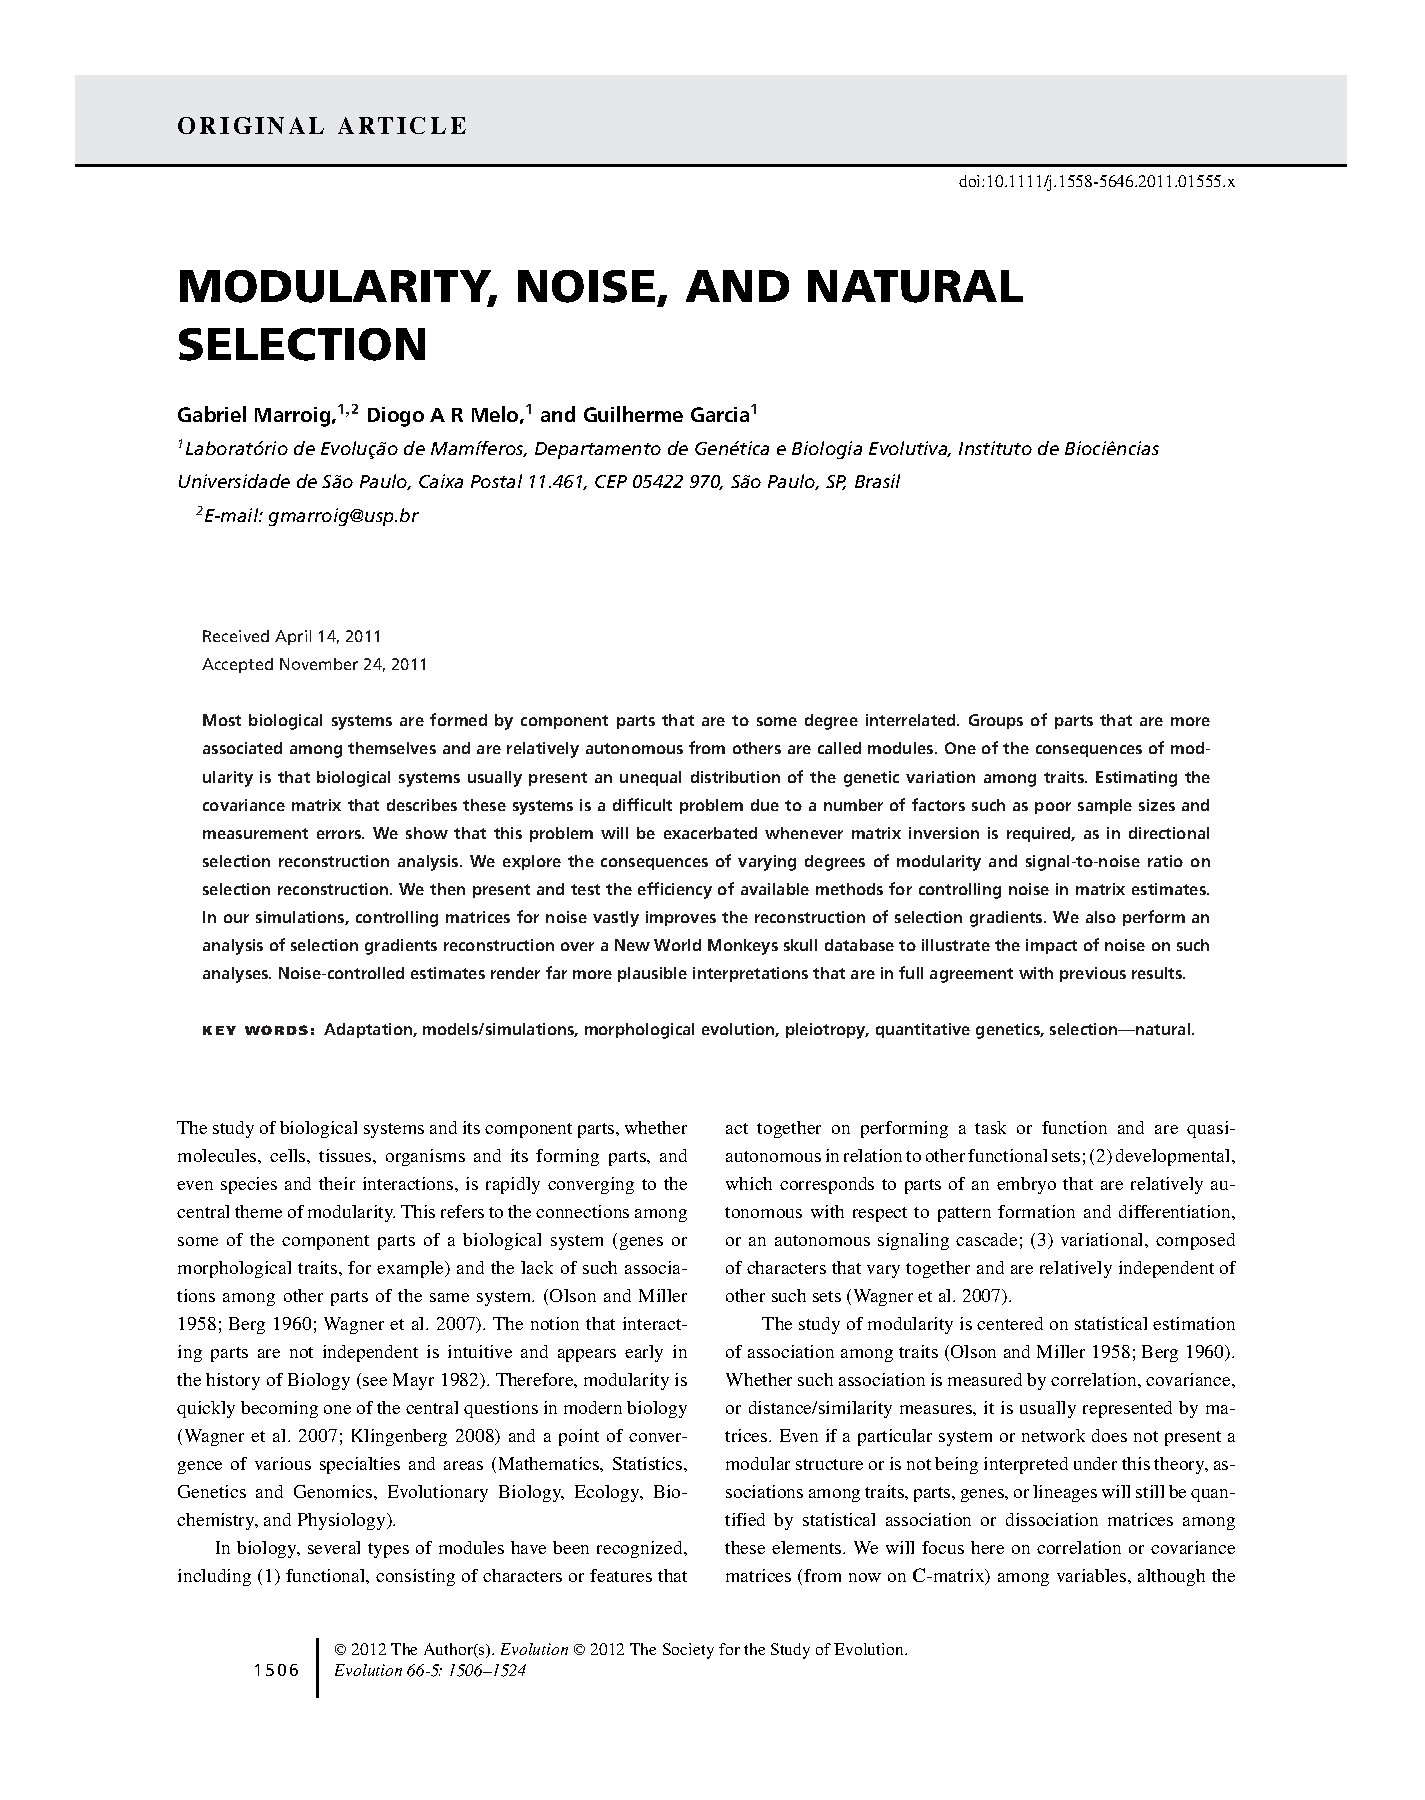
\includepdf[
            pages=-,
            width=189mm,
            height=267.3mm,
            offset=15pt 0pt,
            pagecommand={\pagestyle{plain}}
            ]{Appendix/Marroig2012.pdf}

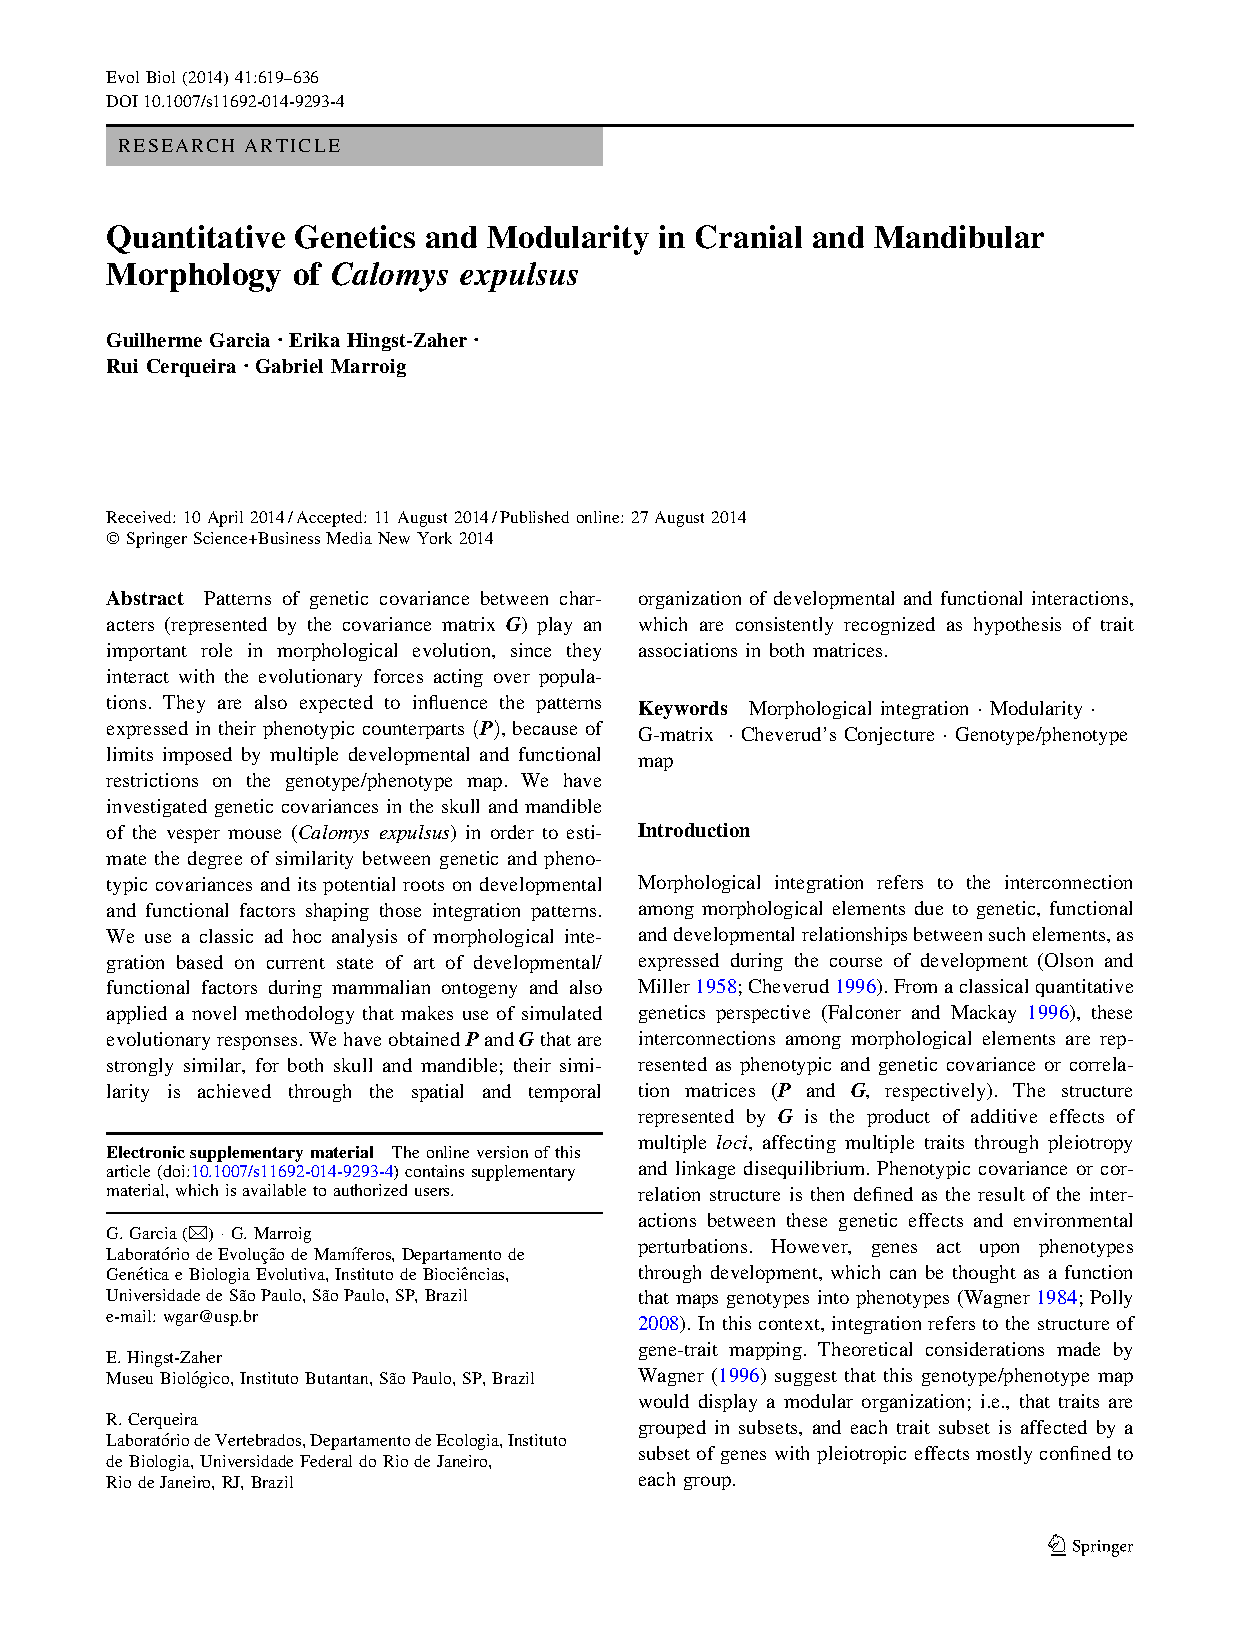
\includepdf[
            pages=-,
            width=189mm,
            height=267.3mm,
            offset=15pt 0pt,
            pagecommand={\pagestyle{plain}}            
            ]{Appendix/Garcia2014.pdf}

\includepdf[
            pages=-,
            width=189mm,
            height=267.3mm,
            offset=15pt 0pt,
            pagecommand={\pagestyle{plain}}            
            ]{Appendix/Melo2015.pdf}

\end{document}
